\documentclass{SNJB}
\usepackage{makeidx}
\usepackage{amssymb}
\usepackage{amsmath}
\usepackage{subfigure}
\usepackage{graphicx}
\usepackage{%
  babel,
  algorithmic,
  algorithm,
  caption
}

\usepackage{url}
\usepackage[breaklinks=true]{hyperref}

\usepackage[]{nomencl}
\renewcommand{\nomname}{Abbreviations}
\makenomenclature

\makeindex

\begin{document}

\title{A Tool for Managing Key Value pairs on Oracle NoSQL Database}

\author{Dahiwadkar Sushank K.\\Kapadni Anjali D.\\}

\newauthor{SDK, ADK }

\new{Dahiwadkar Sushank K. \hspace{0.8cm} B80414227 \\ Kapadni Anjali D. \hspace{2.2cm} B80414274 \\}

\dept{\textbf{Department Of Computer Engineering}}
\supervisor{Prof. M. R. Sanghavi}
\submitdate{2013 - 2014}
\degree{Bachelor of Engineering}
\specialization{Computer Engineering}
\type{Project}
%\type{Seminar}
\hod{Prof. M. R. Sanghavi}

\beforepreface{}

%\end{tabular}


\prefacesection{Acknowledgement}
    \pagenumbering{roman}
    \pagestyle{plain}

%\input{acknowledgement}
\hspace*{0.7in}We would like to acknowledge all the people who have been of the help and assisted us throughout our project work. \\
\hspace*{0.7in}First of all we would like to thank our respected guide Prof. M.R. Sanghavi, Head of Department of Computer Engineering for introducing us throughout features needed. The time-to-time guidance, encouragement, and valuable suggestions received from her are unforgettable in our life. This work would not have been possible without the enthusiastic response, insight, and new ideas from her. We like to thank our mentor Mr. Shirish Joshi working at Persistent Systems Private Limited,Pune.\\
\hspace*{0.7in}We gladly take this opportunity to thank Dr.V.J.Gond, Principal, SNJB�s College of Engineering, Chandwad for providing all the facilities during the progress of dissertation. We are also grateful to all the faculty members of SNJB's College of Engineering for their support and cooperation.\\
\hspace*{0.7in}We would like to thank our lovely parents for time-to-time support and encouragement and valuable suggestions, for the emotional as well as strong support each and every time also for continued loving care and emotional support at every stage of this project. \\
\hspace*{0.7in}We would like to thank our friends for their valuable support and encouragement. In a countless way we have received support and love from all our family members who have constantly encouraged us to achieve new heights. The acknowledgement would be incomplete without mention of the blessing of the Almighty, which helped us in keeping high moral during most difficult period.

\acknowledgeauthor

\prefacesection{Abstract}

\emph{\hspace*{0.7in}Due to huge usage of internet, online data exchange is exponentially increased. Many promising technologies are used to handle the data storage needs in past decades but none of them to be proven sufficient. As a result every industry facing the problem data storagecomes up with in-house solution, and these lead to foundation of standard of NoSQL means not actually SQL (Structured Query Language). So oracle also came up with its product i.e. Oracle NoSQL, which is in developing phase.This project will deal with a Graphical User Interface and Web Services to the Oracle NoSQL Database which will simplify the utility of the Oracle NoSQL.Experimental results show that the proposed solution will be useful for the naive users to use Oracle NoSQL effectively. }
\begin{itemize}
  \item Keywords:
  \\Oracle NoSQL, Big Data, Graphical User Interface, Web Services, Android.
\end{itemize}



% Use following command at the command prompt to display the Abbreviations
% makeindex exemplar.nlo -s nomencl.ist -o exemplar.nls

\newpage
%\addcontentsline{toc}{chapter}{List of Abbreviations}
\printnomenclature
\newpage
\afterpreface

\listoftables
\listoffigures
%\input{glossary}7
\clearpage
\pagenumbering{arabic}
\pagestyle{plain}


\pagestyle{fancy}

\titleformat{\chapter}[display]
{\flushright\normalfont\huge\bfseries}
{\chaptertitlename\ \thechapter}{20pt}{\Huge}


\chapter{Introduction}
\section{Overview}
\hspace*{0.7in} In today's Information Technology world Due to huge usage of internet, online data exchange is exponentially increased. And it is continuously increasing. All this data is generated from social networking websites, E-Commerce portals, and many more Networks. This data includes uploaded images, posted articles, web crawling records, online shopping records, Sensor data etc. As the data increases the need to store that data also increases. And this need of more storage leads to increase in storage cost. This huge data is referred as \textbf{Big Data}.
\\
\hspace*{0.7in} Big data is very large in size which exceeds some petabytes. Managing big data is very tedious job. Many technologies are introduced to manage this big data, but these tools were able to manage the data up to some extent. The data is been stored onto Relational database management systems. But RDBMS are also having their own limitations. As the data increases the operations to manage them also gets more complex. Many operations such as complex queries and joins are tedious to workout. And many more technical issues come up which demands something new for handling this Problem.
\\
\hspace*{0.7in} Many promising technologies were used to handle the data storage needs in past decades but none of them proven to be sufficient. As a result every industry facing the problem of data storage came up with in-house solution, and these lead to foundation of standard of NoSQL, means Not Only SQL (Structured Query Language). NoSQL is the technology which defines many standard and techniques to handle the big data. It does not include structured query language but other techniques to handle the data. NoSQL defines various methods which ensure the data storage over distributed environment. Some NoSQL technologies include MongoDB, CoughDB, and Cassandra etc.
\\
\hspace*{0.7in} Oracle is a leading player in the Database technologies. So oracle also came up with its product i.e. Oracle NoSQL. Oracle NoSQL is a Key Value Paired database. Oracle NoSQL has a strong architecture which ensures all the functions required for storage of Big Data. It is in developing phase. Oracle NoSQL does not have any shell or GUI to simplify the user's need to use the product.
\\
\hspace*{0.7in} This encouraged us for choosing the task to develop a GUI which will be able to manage the Key value pairs on Oracle NoSQL database. Project does not only include the GUI development, but the project is the complete package to manage the Oracle NoSQL Database. The first part of project includes the study of NoSQL and Oracle NoSQL, development of a tool to manage Key Value pairs. The Application is platform independent. The second part of project development includes developing RESTFul web services to manage the Oracle NoSQL database, and developing an Android application to demonstrate the consumption of this web services on Android Platform.
\\
\hspace*{0.7in} This project is a complete package to work with Oracle NoSQL Database.

\section{Brief Description}
\hspace*{0.7in} As the project is developed for managing the database, it covers all the functionalities to manage the Oracle NoSQL Database. Various CRUD functions i.e. create, read, update, delete are included in this project. All the functions are based upon key values. It also includes importing data form CSV file to database and exporting the data to CSV file. RESTFul web services are developed for particular purpose. Web services are been developed for attendance management system. This web services work upon the sensor data which is been stored into the database. The sensor data is generated from bio metrics thumb machine which is used into many organization for employee's attendance purpose. The web services evaluate the information needed to the user and sends to android based device. This android application is specially developed to demonstrate the consumption of this web services and use of Oracle NoSQL for managing Big Data. The Android Application has two options i.e. Daily attendance and Monthly Attendance.

\section{Problem Definition}
\hspace*{0.7in} "Develop a tool for managing Key Value pairs on Oracle NoSQL Database and Web Services to be used on any platform."
\\
\hspace*{0.7in}	The attempt is develop and GUI based application to handle the Oracle NoSQL database which will help all class of users to use Oracle NoSQL. Basically the application is for users who only need to manage the Oracle NoSQL database and not the developers. The application includes all the basic functionalities.
\\
\hspace*{0.7in}	The second part of the project is web services which enables any class of user to use these project functionalities into their application. The project also demonstrates the efficient use to Oracle NoSQL for managing the big data.

\section{Organization of Report}
\begin{itemize}
  \item \textbf{Chapter 1} : Introduction It contains social and technical scenario, introduction  about topic(A Tool for Managing Key-Value Pairs on Oracle NoSQL Database.), basic concept(Provide GUI to perform CRUD as well as Import Export Operation on NoSQL KVStore). Project work, Objective etc. are discussed in this chapter.
\end{itemize}

\begin{itemize}
  \item \textbf{Chapter 2} : Literature Survey A review of the related work in the area of Database Management System is presented in this chapter. The existing approaches to database management on BigData is discussed first, different types of databses are also discussed and finally literature survey is concluded. Also proposed system is discussed.
\end{itemize}

\begin{itemize}
  \item \textbf{Chapter 3} : Software Requirement Specification. It includes introduction, System features, External and internal interface, and Non-functional, other requirements, Goals, objective, Need ,System Implementation Plan, Analysis Model, hardware and software interfaces.
\end{itemize}

\begin{itemize}
  \item \textbf{Chapter 4} : System Design It contain System Architecture, Mathematical Model, UML Diagrams are included in this chapter.
\end{itemize}

\begin{itemize}
  \item \textbf{Chapter 5} : Technical Specification it contains details of technology that are used in project i.e details about java7, java servlet 3.0, glassfish server 4.0, android sdk, html 5, restful webservices etc.
\end{itemize}

\begin{itemize}
  \item \textbf{Chapter 6} : Project Estimate , schedule, Team Structure. It contains details about project estimation cost, scheduling i.e which task is done by which member. It also include Team structure and details about duration required to complete Project.
\end{itemize}

\begin{itemize}
  \item \textbf{Chapter 7} : Software Implementation It gives detail about Algorithm which has been followed for the implementation of system. It also give detail about Mathematical Model.
\end{itemize}

\begin{itemize}
  \item \textbf{Chapter 8} : Software Testing This chapter gives introduction to Testing, introduction to Types of Testing. It also gives test cases that are used in Project for Testing and snapshot of test cases and Test Plan
\end{itemize}

\begin{itemize}
  \item \textbf{Chapter 9} : Result This chapter contain snapshot of system which gives details about how system flow going on and final output is displayed
\end{itemize}



\begin{itemize}
  \item \textbf{Chapter 10} : Conclusion It contains conclusion and Future scope
\end{itemize}


\chapter{Literature Survey}
\section{Database}
\hspace*{0.7in} A database is an organized collection of data. The data are typically organized to model relevant aspects of reality in a way that supports processes requiring this information. For example, modeling the availability of rooms in hotels in a way that supports finding a hotel with vacancies. Database management systems (DBMSs) are specially designed software applications that interact with the user, other applications, and the database itself to capture and analyze data. A general-purpose DBMS is a software system designed to allow the definition, creation, querying, update, and administration of databases. Well-known DBMSs include MySQL, MariaDB, PostgreSQL, SQLite, Microsoft SQL Server, Oracle, SAP HANA, dBASE, FoxPro, IBM DB2, LibreOffice Base and FileMaker Pro. A database is not generally portable across different DBMSs, but different DBMSs can interoperate by using standards such as SQL and ODBC or JDBC to allow a single application to work with more than one database. \cite{1}\\
\hspace*{0.7in} Choosing between databases used to boil down to examining the differences between the available commercial and open source relational databases. The term "database" had become synonymous with SQL, and for a while not much else came close to being a viable solution for data storage. But recently there has been a shift in the database landscape. When considering options for data storage, there is a new game in town: NoSQL databases \cite{2}.

\section{NoSQL}
\hspace*{0.7in} NoSQL databases represent a recent evolution in enterprise application architecture, continuing the evolution of the past twenty years. In the 1990's, vertically integrated applications gave way to client-server architectures, and more recently, client-server architectures gave way to three-tier web application architectures. In parallel, the demands of web-scale data analysis added map-reduce processing into the mix and data architects started avoiding transactional consistency in exchange for incremental scalability and large-scale distribution. The NoSQL movement emerged out of this second ecosystem. NoSQL is often characterized by what it's not depending on whom you ask, it's either not only a SQL-based relational database management system or it's simply not a SQL-based RDBMS. While those definitions explain what NoSQL is not, they do little to explain what NoSQL is. Consider the fundamentals that have guided data management for the past forty years \cite{3}.\\
\hspace*{0.7in} In recent years there was a high demand for massively distributed databases with high partition tolerance but according to the CAP theorem it is impossible for a distributed system to simultaneously provide consistency, availability and partition tolerance guarantees. A distributed system can satisfy any two of these guarantees at the same time, but not all three. For that reason many NoSQL databases are using what is called eventual consistency to provide both availability and partition tolerance guarantees with a maximum level of data consistency. NewSQL is a class of modern relational databases that aims to provide the same scalable performance of NoSQL systems for online transaction processing (read-write) workloads while still using SQL and maintaining the ACID guarantees of a traditional database system. Such databases include Clustrix, EnterpriseDB, NuoDB and VoltDB \cite{1}.
\\
\hspace*{0.7in} The only thing that all NoSQL solutions providers generally agree on is that the term "NoSQL" isn't perfect, but it is catchy. Most agree that the "no" stands for "not only", an admission that the goal is not to reject SQL but, rather, to compensate for the technical limitations shared by the majority of relational database implementations. In fact, NoSQL is more a rejection of a particular software and hardware architecture for databases than of any single technology, language, or product. Relational databases evolved in a different era with different technological constraints, leading to a design that was optimal for the typical deployment prevalent at that time. But times have changed, and that once successful design is now a limitation. You might hear conversations suggesting that a better term for this category is NoRDBMS or half a dozen other labels, but the critical thing to remember is that NoSQL solutions started off with a different set of goals and evolved in a different environment, and so they are operationally different and, arguably, provide better suited solutions for many of today's data storage problems\cite{2}.
\\
\hspace*{0.7in} NoSQL emerged as companies, such as Amazon, Google, LinkedIn and Twitter struggled to deal with unprecedented data and operation volumes under tight latency constraints. Analyzing high-volume, real time data, such as web-site click streams, provides significant business advantage by harnessing unstructured and semi-structured data sources to create more business value. Traditional relational databases were not up to the task, so enterprises built upon a decade of research on distributed hash tables (DHTs) and either conventional relational database systems or embedded key/value stores, such as Oracle's Berkeley DB, to develop highly available, distributed key-value stores. Although some of the early NoSQL solutions built their systems atop existing relational database engines, they quickly realized that such systems were designed for SQL-based access patterns and latency demands that are quite different from those of NoSQL systems, so these same organizations began to develop brand new storage layers. In contrast, Oracle's Berkeley DB product line was the original key/value store; Oracle Berkeley DB Java Edition has been in commercial use for over eight years. By using Oracle Berkeley DB Java Edition as the underlying storage engine beneath a NoSQL system, Oracle brings enterprise robustness and stability to the NoSQL landscape.\cite{3}
\\
\hspace*{0.7in} The next generation of post-relational databases in the 2000s became known as NoSQL databases, including fast key-value stores and document-oriented databases. NoSQL databases are often very fast, do not require fixed table schemas, avoid join operations by storing denormalized data, and are designed to scale horizontally. The most popular NoSQL systems include MongoDB, Couchbase, Riak, memcached, Redis, CouchDB, Hazelcast, Apache Cassandra and HBase, which are all open-source software products.

\subsection{Why NoSQL}
\hspace*{0.7in} NoSQL databases first started out as in-house solutions to real problems in companies such as Amazon Dynamo, Google BigTable, LinkedIn Voldemort, Twitter FlockDB, Facebook Cassandra, Yahoo! PNUTS, and others. These companies didn't start off by rejecting SQL and relational technologies; they tried them and found that they didn't meet their requirements. In particular, these companies faced three primary issues: unprecedented transaction volumes, expectations of low-latency access to massive datasets, and nearly perfect service availability while operating in an unreliable environment. Initially, companies tried the traditional approach: they added more hardware or upgraded to faster hardware as it became available. When that didn't work, they tried to scale existing relational solutions by simplifying their database schema, de-normalizing the schema, relaxing durability and referential integrity, introducing various query caching layers, separating read-only from write-dedicated replicas, and, finally, data partitioning in an attempt to address these new requirements. Although each of these techniques extended the functionality of existing relational technologies, none fundamentally addressed the core limitations, and they all introduced additional overhead and technical tradeoffs. In other words, these were good band aids but not cures.\cite{2}
\\
\hspace*{0.7in} A major influence on the eventual design of NoSQL databases came from a dramatic shift in IT operations. When the majority of relational database technology was designed, the predominant model for hardware deployments involved buying large servers attached to dedicated storage area networks (SANs). Databases were designed with this model in mind: They expected there to be a single machine with the responsibility of managing the consistent state of the database on that system's connected storage. In other words, databases managed local data in files and provided as much concurrent access as possible given the machine's hardware limitations. Replication of data to scale concurrent access across multiple systems was generally unnecessary, as most systems met design goals with a single server and reliability goals with a hot stand-by ready to take over query processing in the event of master failure. Beyond simple failover replication, there were only a few options, and they were all predicated on this same notion of completely consistent centralized data management. Technologies such as two-phase commit and products such as Oracle's RAC were available, but they were hard to manage, very expensive, and scaled to only a handful of machines. Other solutions available included logical SQL statement-level replication, single-master multi-replica log-based replication, and other home-grown approaches, all of which have serious limitations and generally introduce a lot of administrative and technical overhead. In the end, it was the common architecture and design assumptions underlying most relational databases that failed to address the scalability, latency, and availability requirements of many of the largest sites during the massive growth of the Internet \cite{2}.
\\
\hspace*{0.7in} Given that databases were centralized and generally running on an organization's most expensive hardware containing its most precious information, it made sense to create an organizational structure that required at least a 1:1 ratio of database administrators to database systems to protect and nurture that investment. This, too, was not easy to scale, was costly, and could slow innovation. A growing number of companies were still hitting the scalability and performance wall even when using the best practices and the most advanced technologies of the time. Database architects had sacrificed many of the most central aspects of a relational database, such as joins and fully consistent data, while introducing many complex and fragile pieces into the operations puzzle. Schema devolved from many interrelated fully expressed tables to something much more like a simple key/value look-up. Deployments of expensive servers were not able to keep up with demand. At this point these companies had taken relational databases so far outside their intended use cases that it was no wonder that they were unable to meet performance requirements. It quickly became clear to them that they could do much better by building something in-house that was tailored to their particular workloads. These in-house custom solutions are the inspiration behind the many NoSQL products we now see on the market \cite{2}.
\\
\hspace*{0.7in} Furthermore, until recently, integrating NoSQL solutions with an enterprise application architecture required manual integration and custom development; Oracle's NoSQL Database provides all the desirable features of NoSQL solutions necessary for seamless integration into an enterprise application architecture \cite{3}.

\section{Types of NoSQL Databases}
\hspace*{0.7in} In isolation, NoSQL databases are enhanced for retrieve and append operations and also offer functionality beyond record storage. NoSQL databases shows their strong suit with regard to the elastic handling of variable data by document-oriented databases, the graph databases for representing relationships and in the reduction of a database to a container with KVpairs provided by key-value databases. \\
The four types of NoSQL Databases are as follows :
\begin{itemize}
  \item Graph Databases
  \item Document Databases
  \item Columnar Databses
  \item key-Values Stores
\end{itemize}

\subsection{Graph Databases}
\hspace*{0.7in} used which, again, can scale across multiple machines. NoSQL databases do not provide a high-level declarative query language like SQL to avoid overtime in processing. Rather, querying these databases is data-model specific. Many of the NoSQL platforms allow for RESTful interfaces to the data, while other offer query APIs. Examples are Neo4J, InfoGrid, Infinite Graph \cite{8}. Looking at the projection of domain models onto a data structure, there are two dominating schools - the relational way as used for RDBMS and graph and network structures, used for e.g. the Semantic Web. While graph structures in theory are normalizable even in RDBMS, this has serious query performance implications for recursive structures like for instance file trees and network structures like e.g. social graphs, due to the implementation characteristics of relational databases. Every operation over a relationship of a network results in a "join" operation in the RDBMS, implemented as a set-operation between the sets of primary keys for two tables - a slow operation and not scalable over growing numbers of tuples in these tables \cite{4}.
\\
\hspace*{0.7in} There is no existing general consensus on terminology regarding the area of graphs. There exist many different types of graph models. However, there is some effort to create the Property Graph Model, unifying most of the different graph implementations. According to it, information in a Property Graph is modeled using three basic building blocks:
\begin{itemize}
  \item node (a.k.a. vertex)
  \item relationship (a.k.a. edge) - with direction and Type (labeled and directed)
  \item property(a.k.a attribute) on nodes and relationships
\end{itemize}

\begin{figure}[h]
\centering
  % Requires \usepackage{graphicx}
  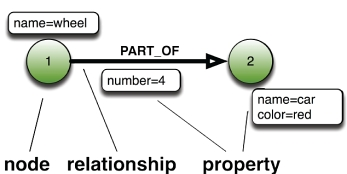
\includegraphics[width=10cm,height=6cm]{L1.jpg}
  \caption{Basic terminology for labeled property graphs}\label{Basic terminology for labeled property graphs}
\end{figure}

\begin{figure}[h]
\centering
  % Requires \usepackage{graphicx}
  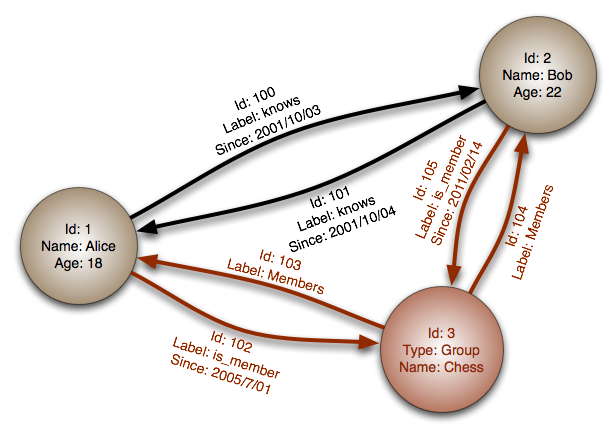
\includegraphics[width=10cm,height=8cm]{L2.png}
  \caption{labeled property graph.}\label{labeled property graph.}
\end{figure}

\begin{itemize}
  \item \textbf{For Example}
\end{itemize}
\hspace*{0.7in} As mentioned before, Social Networks represent just a tiny fraction of the applications of graph databases, as they are easy to understand for this example.
\\
\begin{figure}[h]
\centering
  % Requires \usepackage{graphicx}
  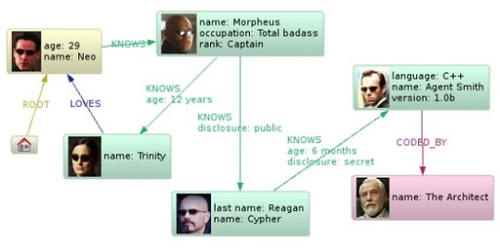
\includegraphics[width=10cm,height=8cm]{L3.jpg}
  \caption{Graph Database exapmle.}\label{Graph Database exapmle.}
\end{figure}
\\

\subsection{Document Databases}
\hspace*{0.7in} These were inspired by Lotus Notes and are similar to key-value stores. The model is basically versioned documents that are collections of other key-value collections. The semi-structured documents are stored in formats like JSON. Document databases are essentially the next level of Key/value, allowing nested values associated with each key.  Document databases support querying more efficiently. Examples are CouchDB, MongoDb \cite{8}. \\
\hspace*{0.7in} The central concept of a document-oriented database is the notion of a Document. While each document-oriented database implementation differs on the details of this definition, in general, they all assume documents encapsulate and encode data (or information) in some standard formats or encodings. Encodings in use include XML, YAML, JSON, and BSON, as well as binary forms like PDF and Microsoft Office documents (MS Word, Excel, and so on). Documents inside a document-oriented database are similar, in some ways, to records or rows in relational databases, but they are less rigid. They are not required to adhere to a standard schema, nor will they have all the same sections, slots, parts, or keys. For example, the following is a document:
$\{$ \\
\hspace*{0.4in} FirstName: "Bob", \\
\hspace*{0.4in} Address: "5 Oak St.", \\
\hspace*{0.4in} Hobby: "sailing" \\
$\}$
\\
\\
A second document might be: \\
\\
$\{$ \\
\hspace*{0.4in} FirstName: "Jonathan",  \\
\hspace*{0.4in} Address: "15 Wanamassa Point Road", \\
\hspace*{0.4in} Children: [ \\
\hspace*{0.4in} $\{$Name: "Michael", Age: 10$\}$,   \\
\hspace*{0.4in} $\{$Name: "Jennifer", Age: 8$\}$,   \\
\hspace*{0.4in} $\{$Name: "Samantha", Age: 5$\}$,   \\
\hspace*{0.4in} $\{$Name: "Elena", Age: 2$\}$   \\
\hspace*{0.4in} ]   \\
$\}$    \\
\\
\hspace*{0.7in} These two documents share some structural elements with one another, but each also has unique elements. Unlike a relational database where every record contains the same fields, leaving unused fields empty; there are no empty 'fields' in either document (record) in the above example. This approach allows new information to be added to some records without requiring that every other record in the database share the same structure \cite{5}.
\subsection{Columnar Databases}
\hspace*{0.7in} These were created to store and process very large amounts of data distributed over many machines. There are still keys but they point to multiple columns. The columns are arranged by column family. Examples are Cassandra, HBase \cite{8}. \\
A column family is a NoSQL object that contains columns of related data. It is a tuple (pair) that consists of a key-value pair, where the key is mapped to a value that is a set of columns. In analogy with relational databases, a column family is as a "table", each key-value pair being a "row". Each column is a tuple (triplet) consisting of a column name, a value, and a timestamp. In a relational database table, this data would be grouped together within a table with other non-related data \cite{6}.\\
Two types of column families exist:
\begin{itemize}
  \item Standard column family: contains only columns
  \item Super column family: contains a map of super columns.
\end{itemize}

\subsection{Key-Value Store Databases}
\hspace*{0.7in} The main idea here is using a hash table where there is a unique key and a pointer to a particular item of data. The Key/value model is the simplest and easiest to implement. But it is inefficient when you are only interested in querying or updating part of a value, among other disadvantages. Examples: Tokyo Cabinet/Tyrant, Redis, Voldemort, Oracle BDB, Amazon SimpleDB, Riak \cite{8}.
\\
\hspace*{0.7in} Key-value stores allow the application to store its data in a schema-less (key, value) pairs. This data is stored in a hash table like data-types, so that each value can be accessed by its major or minor key. Even though such storage facility might not be much effective as they provide single way to access the values, but excludes the need for a fixed data model.
\\
\begin{figure}[h]
\centering
  % Requires \usepackage{graphicx}
  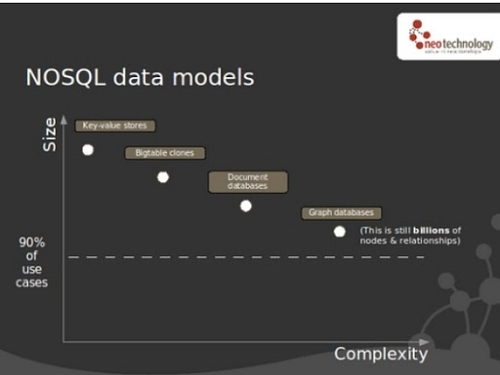
\includegraphics[width=10cm,height=8cm]{L4.jpg}
  \caption{NoSQL Data Models}\label{NoSQL Data Models}
\end{figure}
\\

\subsubsection{Oracle Key Value Pair NoSQL Database}
\hspace*{0.7in} Oracle NoSQL Database provides multi-terabyte distributed key/value pair storage that offers scalable throughput and performance. That is, it services network requests to store and retrieve data which is organized into key-value pairs. Oracle NoSQL Database services these types of data requests with a latency, throughput, and data consistency that is predictable based on how the store is configured. Oracle NoSQL Database offers full Create, Read, Update and Delete (CRUD) operations with0 adjustable durability guarantees. Oracle NoSQL Database is designed to be highly available, with excellent throughput and latency, while requiring minimal administrative interaction. \\
\hspace*{0.7in} Oracle NoSQL Database provides performance scalability. If you require better performance, you use more hardware. If your performance requirements are not very steep, you can purchase and manage fewer hardware resources. Oracle NoSQL Database is meant for any application that requires network-accessible key-value data with user-definable read/write performance levels. The typical application is a web application which is servicing requests across the traditional three-tier architecture: web server, application server, and back-end database. In this configuration, Oracle NoSQL Database is meant to be installed behind the application server, causing it to either take the place of the back-end database, or work alongside it. To make use of Oracle NoSQL Database, code must be written (using Java or C) that runs on the application server. An application makes use of Oracle NoSQL Database by performing network requests against Oracle NoSQL Database's key-value store, which is referred to as the KVStore. The requests are made using the Oracle NoSQL Database Driver, which is linked into your application as a Java library (.jar file), and then accessed using a series of Java APIs. \\
\begin{itemize}
    \item The KVStore :
\end{itemize}
\hspace*{0.7in} The KVStore is a collection of Storage Nodes which host a set of Replication Nodes. Data is spread across the Replication Nodes. The store contains multiple Storage Nodes. Every Storage Node hosts one or more Replication Nodes as determined by its capacity. \\
\begin{itemize}
    \item Replication Nodes and Shards :
\end{itemize}
\hspace*{0.7in} At a very high level, a Replication Node can be thought of as a single database which contains key-value pairs. Replication Nodes are organized into shards. A shard contains a single Replication Node, called the master node, which is responsible for performing database writes. The master node copies those writes to the other Replication Nodes in the shard, called the replicas. These replicas obtain a full copy of the data from the corresponding master node and are used to service read-only operations. Although there can be only one master node at any given time, any of the members of the shard are capable of becoming a master node.
\\
\begin{itemize}
    \item Replication Factor :
\end{itemize}
\hspace*{0.7in} The number of nodes belonging to a shard is called its Replication Factor. The larger a shard's Replication Factor, the faster its read throughput (because there are more machines to service the read requests) but the slower its write performance (because there are more machines to which writes must be copied).
\\
\begin{itemize}
    \item Partitions :
\end{itemize}
\hspace*{0.7in} Each shard contains one or more partitions. Key-value pairs in the store are organized according to the key. Keys, in turn, are assigned to a partition. Once a key is placed in a partition, it cannot be moved to a different partition.
\\
\begin{itemize}
    \item KVLite :
\end{itemize}
\hspace*{0.7in} KVLite is a simplified version of Oracle NoSQL Database. It provides a single-node store that is not replicated. It runs in a single process without requiring any administrative interface. You configure, start, and stop KVLite using a command line interface.

\begin{itemize}
    \item Architecture of Key Value Pair NoSQL Database
\end{itemize}

\begin{figure}[h]
\centering
  % Requires \usepackage{graphicx}
  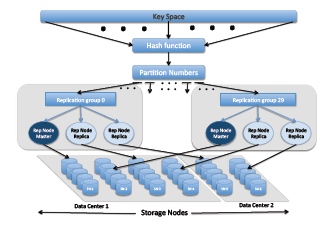
\includegraphics[width=10cm,height=8cm]{A1.png}
  \caption{Architecture of Key Value Pair NoSQL Database}
  \label{Architecture of Key Value Pair NoSQL Database}
\end{figure}

\begin{itemize}
    \item The CAP Theorem of NoSQL Database
\end{itemize}
\hspace*{0.7in} Despite the high demand in recent years for massively distributed databases with high partition fault-tolerance, the CAP theorem stipulates that it is actually impossible for a distributed system to provide consistency, availability and partition fault-tolerance guarantees simultaneously; a distributed system can satisfy at most any two of these guarantees at the same time, but not all three. These guarantees can be understood as follows:
\\
\begin{figure}[h]
\centering
  % Requires \usepackage{graphicx}
  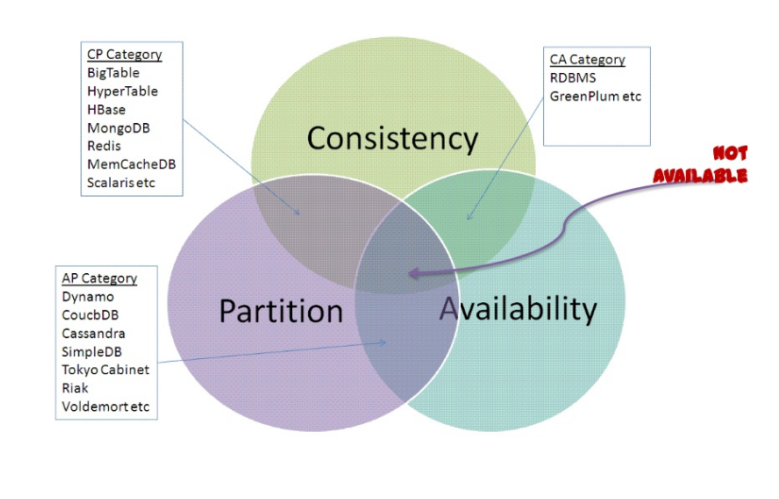
\includegraphics[width=10cm,height=8cm]{C1.png}
  \caption{CAP Theorem of NoSQL}\label{CAP Theorem of NoSQL}
\end{figure}
\\
\textbf{Consistency }: Concurrently executing queries see the same valid and consistent data at the same time. \\
\textbf{Availability }: This is a guarantee that every request receives a response about whether it succeeded or failed. \\
\textbf{Partition-tolerance }: Also known as fault-tolerance, this is a guarantee that the system continues to operate despite arbitrary message loss.\\

\hspace*{0.7in} Because no distributed system is capable of satisfying all three guarantees at the same time, a trade-off must be made. While traditional databases make that decision for us, NoSQL databases provide these guarantees as tuning options. Database vendors must always decide which two to prioritize. The options are as follows:
\begin{enumerate}
  \item Availability is compromised in favour of consistency and partition-tolerance.
  \item Partition-tolerance is forfeited in favour of consistency and availability.
  \item Consistency is compromised but systems are always available and can work when parts are partitioned.
\end{enumerate}

Traditional SQL databases place a high priority on consistency and fault-tolerance and have generally as a result chosen to go with the first option above and forfeit high availability. NoSQL databases frequently leave that decision to the application operations team and provide configuration options so that the preferred options can be chosen based on the application use case

\begin{itemize}
    \item NoSQL in Practice
\end{itemize}
There are many products that now claim to be part of the NoSQL database market, far too many to mention here or describe in any detail.
\\
\begin{figure}[h]
\centering
  % Requires \usepackage{graphicx}
  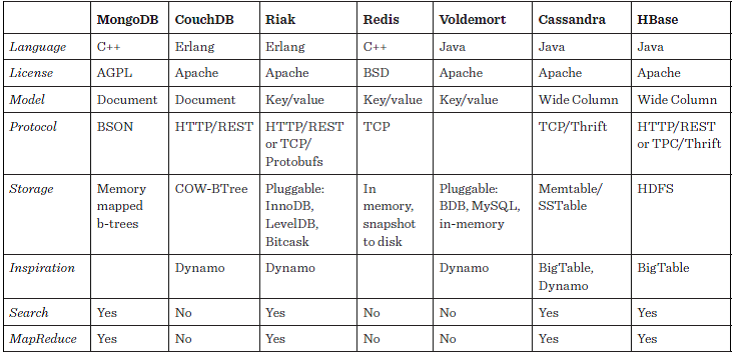
\includegraphics[width=13cm,height=7cm]{T1.png}
  \caption{NoSQL in Practice}\label{NoSQL in Practice}
\end{figure}

\section{Characteristics of NoSQL Databases}
\begin{itemize}
  \item Auto-sharding - A NoSQL database automatically spreads data across servers, without requiring applications to participate. Servers can be added or removed from the data layer without application downtime, with data (and I/O) automatically spread across the servers. Most NoSQL databases also support data replication, storing multiple copies of data across the cluster, and even across data centers, to ensure high availability and support disaster recovery. A properly managed NoSQL database system should never need to be taken offline, for any reason, supporting 24x365 continuous operations of applications.

  \item Unstructured Database.

  \item Distributed query support - "Sharding" a relational database can reduce, or eliminate in certain cases, the ability to perform complex data queries. NoSQL database systems retain their full query expressive power even when distributed across hundreds of servers.

  \item Integrated caching - To reduce latency and increase sustained data throughput, advanced NoSQL database technologies transparently cache data in system memory. This behavior is transparent to the application developer and the operations team, compared to relational technology where a caching tier is usually a separate infrastructure tier that must be developed to, deployed on separate servers, and explicitly managed by the ops team.
\end{itemize}

\chapter{Software Requirement Specification}
\section{Introduction}
\subsection{Purpose}
\hspace*{0.7in} The purpose of this section is to describe "A Tool For Managing Key Value Pairs on Oracle NoSQL". This document contains the functional and non-functional requirements of the project. The recent problem of exponentially growing data and to store and manage is needed to be solved. As a solutions new technologies are been introduced in the market by various vendors. But again using these technologies needs trainings to users. As these technologies does not resemble in any way with the traditional technologies. So the purpose is to make this new introduced Oracle NoSQL, familiar with the user by providing various tools to manage this database for user's purpose.

\subsection{Project Scope}
\hspace*{0.7in} A Tool for Managing Key Value Pairs on Oracle NoSQL is basically a application through which the user can make fundamental operations on Oracle NoSQL Database. Project provides various CRUD functions and Import and Export. Here user has to provide the key and its value either one by one or into chunk from CSV File. The project also provides RESTFul web services which provide all the functionalities for managing Oracle NoSQL Database. The project has an Android Application which is used for Attendance check for the users of particular organization. The application can be used in:
\begin{enumerate}
  \item Performing basic operations on Oracle NoSQL Database.
  \item Into an organization where Oracle NoSQL is used.
  \item The RESTFul web services can be used by any application which needs to use the Oracle NoSQL Database functionalities.
  \item The Attendance check application can be used by organizations having Biometric thumb scan machine for attendance.
\end{enumerate}

\subsection{Need}
\hspace*{0.7in} The system is needed because Oracle NoSQL database does not have any Command Line Interface or Graphical User Interface for managing the database. So the system provides GUI and RESTFul web services which make the ease to user, to handle the Oracle NoSQL database. The RESTFul web services are intended to provide project functionalities on any platform or any class of user.

\subsection{Benefits}
\hspace*{0.7in} It is stated that any database should provide ease to users to make operations effort less and efficient. So this project is intended to reduce the user's efforts for managing Oracle NoSQL database by providing GUI and RESTFul web services for the same.
\subsection{Objectives}
\hspace*{0.7in} The objective behind implementing this application is to make a tool which could make the interaction of user easier with Oracle NoSQL database. This application is is new access mechanism for managing database. The application provides interactive and intuitive interface to the user. The Project also provides RESTFul web services which can be used on any platform who needs to make use of Oracle NoSQL Database.

\subsection{User Classes and Characteristics}
\hspace*{0.7in} Users of the system might be any person who needs to interact or use the Oracle NoSQL Database. The user must have basic knowledge of the Key Value Pair based Oracle NoSQL database and computer. Administrators of the system must have more knowledge about the internal modules of the system and are able to rectify small problems that may arise due to disk crashes, network failure, power failure and other catastrophes. Friendly user interface, help options and user guide must be sufficient to educate the user on how to use this product without any problem or difficulties.

\subsection{Operating Environment}
\hspace*{0.7in} The project is an online application, which is deployed on the application server. So the application can be accessed and used from any platform having internet connectivity. The RESTFul web services are free to use on any platform, but mostly the RESTFul web services are intended to use on mobile platform or on the platform where low data is to be handled. And the attendance check application works on Android Platform.

\subsection{Assumptions and Dependencies}
\begin{itemize}
  \item The application is intended to be used for managing big data, the user must have fast internet connectivity on his/ her system.
  \item The user who wants to use the RESTFul web services must know how to use the web services on mobile or any other platform.
  \item The most important is that, any user who needs to use the system must have basic knowledge of the Oracle NoSQL Database.
\end{itemize}

%****************************************************************************************************************************

\section{System Features}
\begin{itemize}
  \item Connect To Store
\begin{figure}[h]
\centering
  % Requires \usepackage{graphicx}
  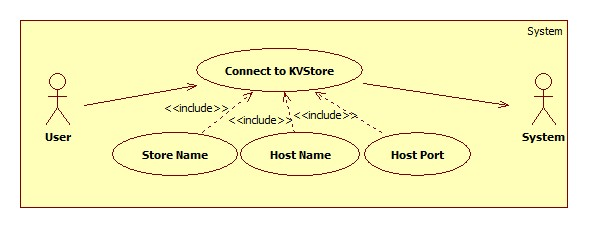
\includegraphics[width=13cm,height=7cm]{Fig1.jpg}
  \caption{Connect To Store}\label{Connect To Store}
\end{figure}
\end{itemize}

\newpage
\begin{itemize}
  \item Insert Data Into Store
\begin{figure}[h]
\centering
  % Requires \usepackage{graphicx}
  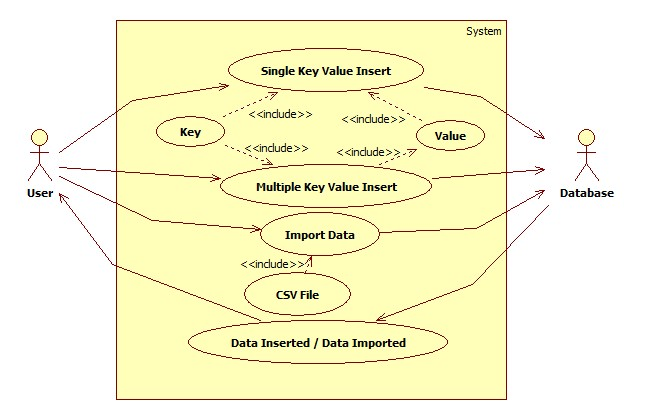
\includegraphics[width=11.5cm,height=8cm]{Fig2.jpg}
  \caption{Insert Data Into Store}\label{Insert Data Into Store}
\end{figure}
\end{itemize}

\begin{itemize}
  \item Display Data
\begin{figure}[h]
\centering
  % Requires \usepackage{graphicx}
  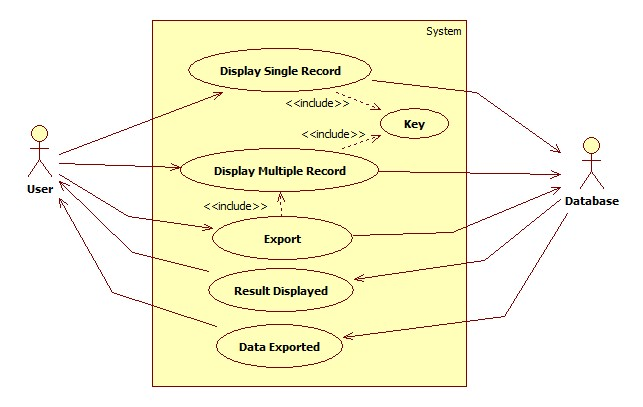
\includegraphics[width=11.5cm,height=8cm]{Fig3.jpg}
  \caption{Display Data}\label{Display Data}
\end{figure}
\end{itemize}

\newpage
\begin{itemize}
  \item Delete Data
\begin{figure}[h]
\centering
  % Requires \usepackage{graphicx}
  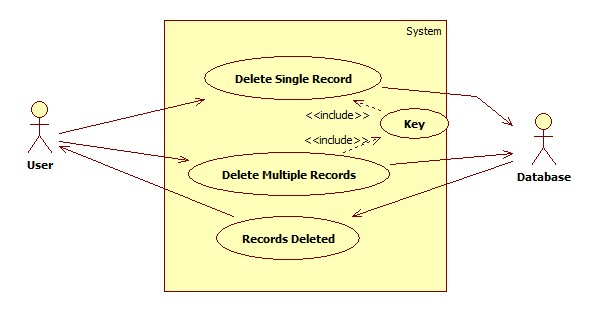
\includegraphics[width=11.5cm,height=9cm]{Fig4.jpg}
  \caption{Delete Data}\label{Delete Data}
\end{figure}
\end{itemize}

\begin{itemize}
  \item Update Data
\begin{figure}[h]
\centering
  % Requires \usepackage{graphicx}
  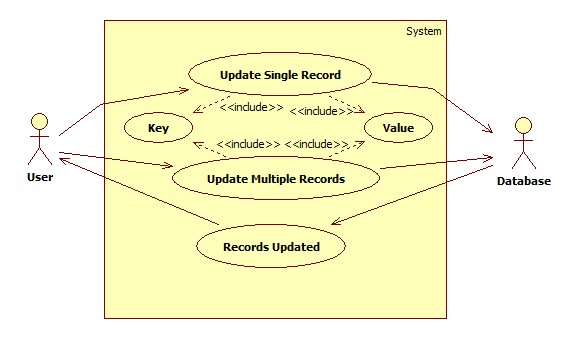
\includegraphics[width=11.5cm,height=7cm]{Fig5.jpg}
  \caption{Update Data}\label{Update Data}
\end{figure}
\end{itemize}

\newpage
\begin{itemize}
  \item Import/Export
\begin{figure}[h]
\centering
  % Requires \usepackage{graphicx}
  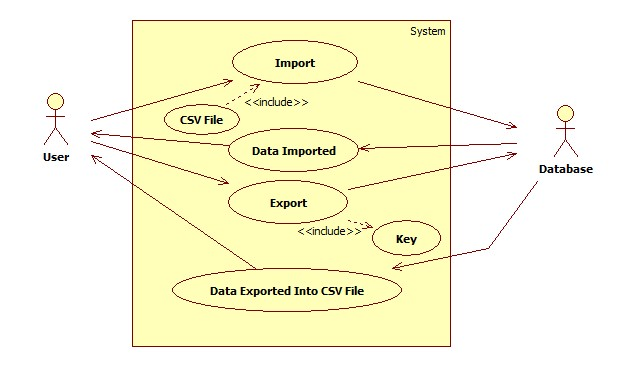
\includegraphics[width=11.5cm,height=8cm]{Fig6.jpg}
  \caption{Import/Export}\label{Import/Export}
\end{figure}
\end{itemize}

\begin{itemize}
  \item Daily Attendance Check
\begin{figure}[h]
\centering
  % Requires \usepackage{graphicx}
  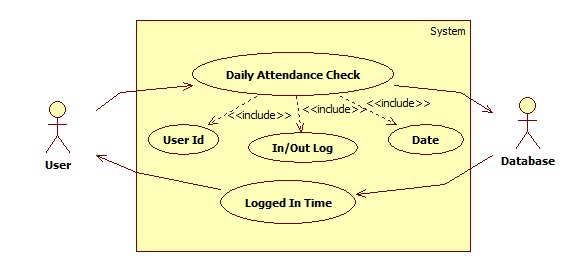
\includegraphics[width=11.5cm,height=7cm]{Fig7.jpg}
  \caption{Daily Attendance Check}\label{Daily Attendance Check}
\end{figure}
\end{itemize}

\newpage
\begin{itemize}
  \item Monthly Attendance Check
\begin{figure}[h]
\centering
  % Requires \usepackage{graphicx}
  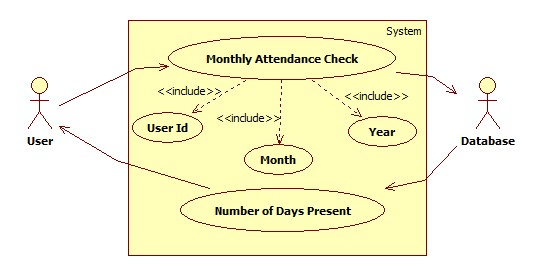
\includegraphics[width=11.5cm,height=7cm]{Fig8.jpg}
  \caption{Monthly Attendance Check}\label{Monthly Attendance Check}
\end{figure}
\end{itemize}

%***************************************************************************************8
\section{External Interface Requirements}
\subsection{User Interfaces}
\begin{itemize}
  \item Home Screen :
\end{itemize}
After starting the application home screen should appears. Home screen has various options including insert, display, update, delete, import and export. But for performing any of this operation the application needs to be connected to the KVStore. For this purpose application asks to user for three options i.e. Store Name, Host Name on which the database is installed and the Host Port on which the database service is running. After getting these parameters the application would connect to database server. And the session for that user should be initialized.

\begin{itemize}
  \item Insert Record :
\end{itemize}
Using this option the user can insert either single Key Value pair or Multiple Key Value pairs into the database. For single Key Value Pair insertion user needs to enter Major Key Component, Minor Key Component and Value. And for multiple Key Value Pairs insertion first user needs to enter Major Key Component and number of Minor Key Component for same, followed by this number of Minor Key Components would have to be inserted and Values for them respectively.

\begin{itemize}
  \item Display Record :
\end{itemize}
This option is used for either single or multiple Key Value Pair display. For single Key Value Pair display user needs to enter the Major Key Component and Minor Key Component of which the value is to be displayed. And for multiple Key Value pairs display user only needs to enter Major Key Component.

\begin{itemize}
  \item Delete Record :
\end{itemize}
This option is used to delete single or multiple Key Value pair from database. For single value deletion user needs to enter Major Key Component and Minor Key Component and for deletion of multiple records user has to enter Major Key Component only.

\begin{itemize}
  \item Update Record :
\end{itemize}
Using this option the user can update the existing records into database. For updating single key value pair user has to enter Major Key Component, Minor Key Component and Value for them. And for updating multiple Key Value pair user has to enter Major Key Component its Minor Key Components and their respected values.

\begin{itemize}
  \item Import :
\end{itemize}
This option should provide the functionality of importing data from CSV file to Oracle NoSQL Database. Here very firstly a CSV file is uploaded to the server. And after that user has to specify Major Key Component and Minor Key Component for that file and user also has to specify that which field from the file is to be relate with Minor Key Component.

\begin{itemize}
  \item Export :
\end{itemize}
Here the user can export the data to CSV file from the database. Very firstly the user has to specify Major Key Component by which he/she would get multiple records and after that user can download that file.

\begin{itemize}
  \item Android Interface for Attendance Check :
\end{itemize}
Using this application the user can check daily as well as monthly attendance. Here the user first needs to connect to database and after that user has to specify userid, In/Out log and date for daily attendance check, and userid, month and year for monthly attendance check.

\subsection{Hardware Interfaces}
\begin{itemize}
  \item Intel Core 2 Duo or higher processor.
  \item Android device with Ginger bread version or higher.
  \item Android device with more than 125 mb RAM.
  \item For deployment of server application the server should be good configuration.
\end{itemize}

\subsection{Software Interfaces}
\begin{itemize}
  \item Any operating system where java can be installed.
  \item Apache tomcat or Glassfish server.
  \item Any Internet browser.
  \item Android operating system.
\end{itemize}

\section{Nonfunctional Requirements}

\subsection{Performance Requirements}
\begin{itemize}
  \item The server must be able to handle all the requests incoming from the clients.
  \item Network bandwidth must be properly managed while the big CSV file is uploaded to the server.
  \item While retrieving multiple Key Value from the database server, the records must be retrieved into batches so that network would not get jammed.
  \item On android device the application must not take more space into internal memory and RAM.
  \item The client must operate at less internet speed.
\end{itemize}

\subsection{Safety Requirements}
\begin{itemize}
  \item UPS: in case of power failure the system requires UPS.
  \item Hard Disk:  the database server must have enough space to store the Data.
  \item The network at the database server side must be properly managed so that it should not crash during the operations are in progress.
\end{itemize}

\subsection{Software Quality Attributes}
\begin{itemize}
  \item Data Security : The data stored at the database server is safe as the Oracle NoSQL takes care of it.
  \item Adaptability : the system must be able to adapt the changes made onto the device. In case if the system software is updated then the application must also adapt those changes.
  \item Availability : availability defines that whenever the application is needed that time user must get the service.
  \item Correctness : every time the data is accessed that time correct data should be provided.
  \item Flexibility : the application should be flexible with any class of user.
  \item Maintainability : the system should not need more maintenance as the end user is not expertise to do so.
  \item Reliable: the user can be reliable on the system, as the system is reliable.
  \item Reusability: the code of application is reusable. The RESTFul web can be reused into other applications.
  \item Robustness: the application can be operate into any device environment.
  \item Testability: the system can be exposed to the test all its functionalities.
\end{itemize}
 %************************************************************************************

\section{Analysis Model}
\subsection{Class Diagrams}
\hspace*{0.7in} Class diagram in the unified modeling language(UML) is a type of static structure  diagram that describes the structure of a system by showing the system's classes, their attributes ,and the relationship between the classes .It is the main building block in object oriented modeling. It is being used for both general conceptual modeling of the systematic of the application, and for detailed modeling translating into programming code \\
\begin{figure}[h]
\centering
  % Requires \usepackage{graphicx}
  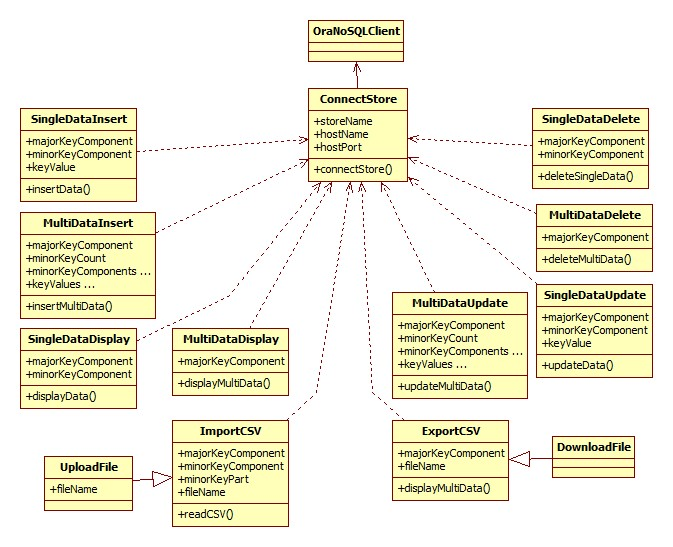
\includegraphics[width=17cm,height=13cm]{Fig9.jpg}
  \caption{Class Diagrams}\label{Class Diagrams}
\end{figure}

\newpage
\section{System Implementation Plan}
There are many important phases for implementation. Following are some important phases and task of implementation.
\begin{itemize}
  \item The main phase to study the NoSQL standard.
  \item Followed by that to Study the Oracle NoSQL and its Architecture in detail.
  \item Understand the use case for which the system is to be implemented.
  \item After understanding the use case proper plan is to created.
  \item So according to plan very first the GUI is to be decided. Various functions will be decided which are to be performed by the system. Based on this function further implementation will be done.
  \item Taking consideration the implementation phase, all the necessary software required for implementation should be installed on the machine.
  \item After the GUI based application is completed, test its functionalities. If all functionalities are up to the mark then proceed to the next phase or remove the errors or bugs.
  \item The next phase is to implement the RESTFul web services. For this purpose, first understand the use case and accordingly start the implementation.
  \item Test the web services, if they are according to use case they move further or again check the functionalities and correct it.
  \item Next step is to implement the Android Application which will consume the RESTFul web services.
  \item After completing the entire above tasks the application is ready to be used.
\end{itemize}

\subsection{Description of Implementation}
\begin{itemize}
  \item The system must be developed into phases as described above.
  \item The system should follow prototype model.
  \item Here none of the prototype depends upon each other, so can be developed in parallel. Development in parallel will reduce the time to develop the project and also the implementation cost.
\end{itemize}



\chapter{System Design}
\section{System Architecture}

\begin{figure}[h]
\centering
  % Requires \usepackage{graphicx}
  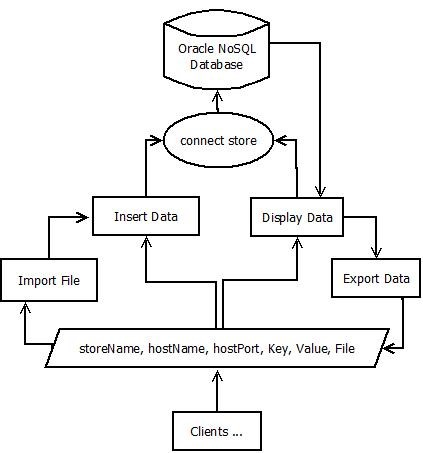
\includegraphics[width=14cm,height=13cm]{Fig10.jpg}\\
  \caption{System Architecture} \label{System Architecture}
\end{figure}

Brief summary of the software architecture is described below in the form of following UML Diagrams :
\begin{enumerate}
  \item State transition diagram
  \item Sequence diagram
  \item Collaboration diagram
  \item Package diagram
  \item Component diagram
  \item Deployment diagram
\end{enumerate}

\subsubsection{State transition diagram}
\hspace*{0.7in} A state machine diagram models the behavior of a single object specifying the sequence of an event that an object goes through during lifetime in response to events. Elements used in state diagram are Initial state, state, transition, history state, final state, signals etc. The most common purpose for which you will use state machines is to model the lifetime of an object, especially instance of classes, use cases and the system as a whole.
\\
\begin{figure}[h]
\centering
  % Requires \usepackage{graphicx}
  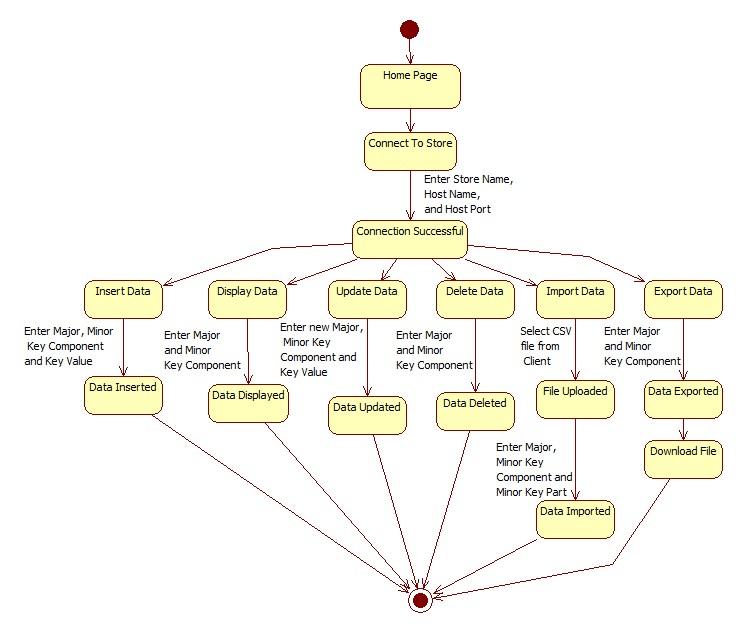
\includegraphics[width=13cm,height=10.5cm]{Fig11.jpg}\\
  \caption{State Transition For User}
  \label{State Transition For User}
\end{figure}

\newpage
\begin{itemize}
  \item GUI based  System :
\end{itemize}

\begin{figure}[h]
\centering
  % Requires \usepackage{graphicx}
  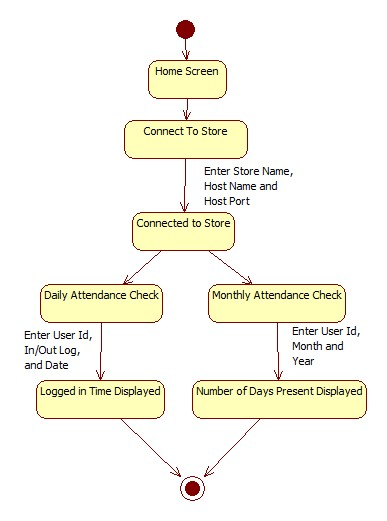
\includegraphics[width=8cm,height=13cm]{Fig12.jpg}\\
  \caption{Attendance check  System}
  \label{Attendance check  System}
\end{figure}

\subsubsection{Sequence diagram}
\hspace*{0.7in} A sequence diagram in Unified Modelling Language (UML) is a kind of interaction diagram that shows how processes operate with one another and in what order. It is a construct of a Message Sequence Chart. A sequence diagram shows, as parallel vertical lines (lifelines), different processes or objects that live simultaneously, and, as horizontal arrows, the messages exchanged between them, in the order in which they occur. This allows the specification of simple runtime scenarios in a graphical manner.
\begin{figure}[h]
\centering
  % Requires \usepackage{graphicx}
  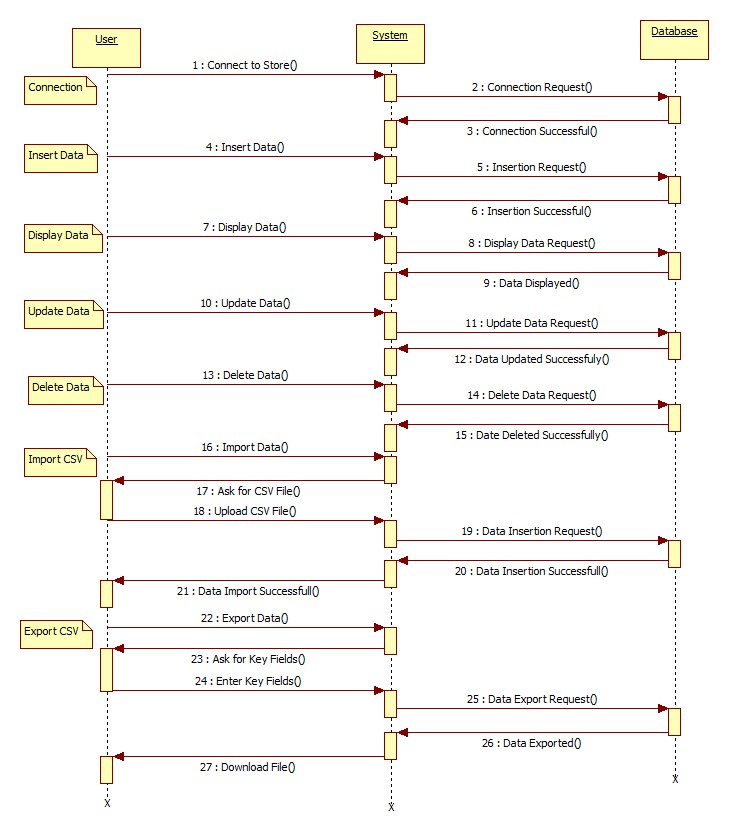
\includegraphics[width=15cm,height=15cm]{Fig13.jpg}\\
  \caption{Sequence Diagram}
  \label{Sequence Diagram}
\end{figure}

\newpage
\begin{itemize}
  \item GUI based  System :
\end{itemize}
\begin{figure}[h]
\centering
  % Requires \usepackage{graphicx}
  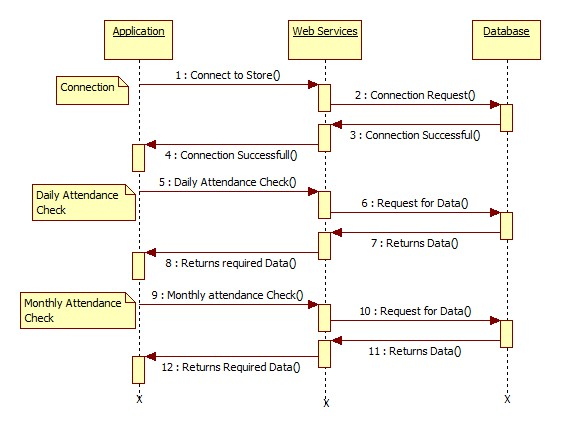
\includegraphics[width=13cm,height=8cm]{Fig14.jpg}\\
  \caption{Attendance check  System}
  \label{Attendance check  System}
\end{figure}

\newpage
\subsubsection{Collaboration diagram}
\hspace*{0.7in} A collaboration diagram describes interactions among objects in terms of sequenced messages. Collaboration diagrams represent a combination of information taken from class, sequence, and use case diagrams describing both the static structure and dynamic behavior of a system.

\begin{figure}[h]
\centering
  % Requires \usepackage{graphicx}
  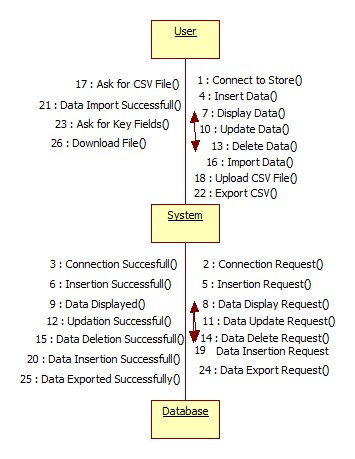
\includegraphics[width=7cm,height=8cm]{Fig15.jpg}\\
  \caption{Collaboration Diagram}
  \label{Collaboration Diagram}
\end{figure}
\newpage
\begin{itemize}
  \item GUI based  System :
\end{itemize}

\begin{figure}[h]
\centering
  % Requires \usepackage{graphicx}
  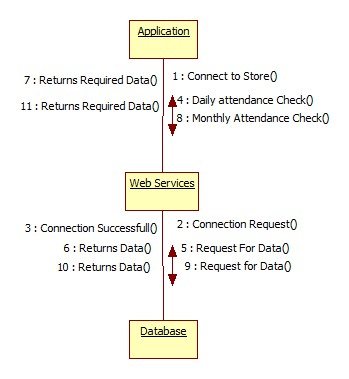
\includegraphics[width=6cm,height=8cm]{Fig16.jpg}\\
  \caption{Attendance check  System}
  \label{Attendance check  System}
\end{figure}

\subsubsection{Package diagram}
\hspace*{0.7in} Package is general purpose mechanism for organizing elements into groups. Every package must have a name that distinguishes it from other packages. Package name must be unique within its enclosing package .A name is a textual string .That name alone is known is known as simple name. A path name is package name prefixed by name of package lives.
\\
\begin{figure}[h]
\centering
  % Requires \usepackage{graphicx}
  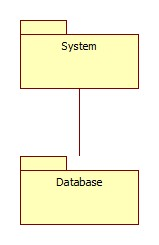
\includegraphics[width=4cm,height=5cm]{Fig17.jpg}\\
  \caption{Package Diagram}
  \label{Package Diagram}
\end{figure}
\\
\newpage
\begin{itemize}
  \item GUI based  System :
\end{itemize}
\begin{figure}[h]
\centering
  % Requires \usepackage{graphicx}
  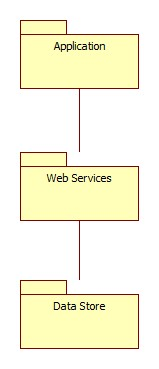
\includegraphics[width=5cm,height=8cm]{Fig18.jpg}\\
  \caption{Attendance check  System}
  \label{Attendance check  System}
\end{figure}

\subsubsection{Deployment Diagram}
\hspace*{0.7in} Deployment diagram represents the deployment view of a system. It is related to the component diagram. Because the components are deployed using the deployment diagrams. A deployment diagram consists of nodes. Nodes are nothing but physical hardware used to deploy the application.

\begin{figure}[h]
\centering
  % Requires \usepackage{graphicx}
  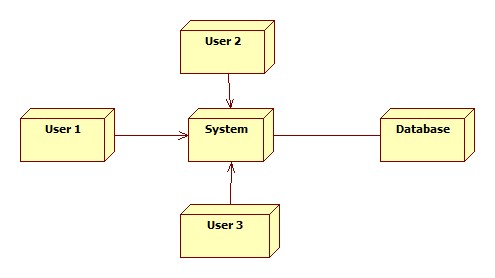
\includegraphics[width=8cm,height=7cm]{Fig19.jpg}\\
  \caption{Deployment Diagram}
  \label{Deployment Diagram}
\end{figure}
\newpage
\begin{itemize}
  \item GUI based  System :
\end{itemize}

\begin{figure}[h]
\centering
  % Requires \usepackage{graphicx}
  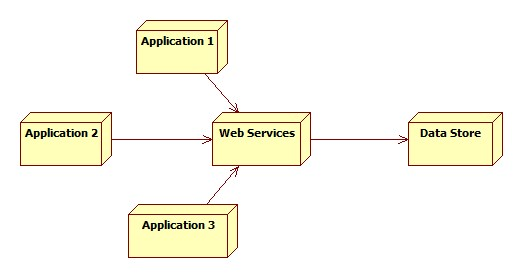
\includegraphics[width=8cm,height=7cm]{Fig20.jpg}\\
  \caption{Attendance check  System}
  \label{Attendance check  System}
\end{figure}


\chapter{Technical Specification}
\section{Technology used for the project}
\begin{itemize}
  \item Java 7 :
\end{itemize}
Java is a complete package for application and generic programming. Java is used to develop various kind of application from console to high end applications. We have used Java Software Development Toolkit Version 7 for our project development.
\\
\begin{itemize}
  \item Java Servlet 3.0 :
\end{itemize}
Java servlet is a part of Java EE community project. Servlet provide an full package for web application development. Java servlets is a technology which works at the server in web applications. Servlets are used for handling the reuests from various clients. Servlets is having strong set of functions for managing the web applications. Every functionality of java SE and java EE is embedded or can be used with java servlet. Servlet has two functions namely doGet() and doPost() which manage all the request from clients. Servlets can be of type Generic servlet or HTTP servlets. We have used HTTP servlets for our project development. Java servlets comes into the package i.e. javax.servlet.*; 
\\
\begin{itemize}
  \item Glassfish Server 4.0:
\end{itemize}
Glassfish is world's first java EE 7 application server. Application server is for deployment of various applications which are developed for web. Glassfish server is used to host to deploy the application which is developed under java EE. Glassfish has excellent support for Java EE 7 applications.  Our project is tested and deployed on Glassfish server 4.0 which is provided along with Netbeans IDE 7.4.
\\
\begin{itemize}
  \item Android SDK:
\end{itemize}
Android Software development toolkit provides platform for android developers where they can develop android applications.  Android SDK comes along with all the necessary library files which are used for android application development. SDK provides development from very older version to latest version. The application developed can work on Android version 2.2 to latest version 4.4.
\\
\begin{itemize}
  \item HTML 5:
\end{itemize}
Hyper Text Markup Language is an language which is used to develop Graphical user interface for web applications. HTML 5 is latest version which has all new features. The GUI for web application is this project is developed under HTML 5.
\\
\begin{itemize}
  \item RESTful web services:
\end{itemize}
REpresentational State Transfer (REST) is a technology which provides a  stateless client-server architecture in which the web services are viewed as resources and can be identified by their URLs. Web service clients that want to use these resources access a particular representation by transferring application content using a small globally defined set of remote methods that describe the action to be performed on the resource. In Simple language RESTful web services are a kind of web applications which acen be accssed form any type of client, RESTful web services provide platform independent service to all clients. We developed web services which are used to for managing KVStore Oracle NoSQL Database.


 

\chapter{Project Estimate, Schedule And Team Structure }
\section{System Implementation Plan}
\hspace*{0.7in} There are many important phases for implementation. Following are important phases and tasks of implementation: \\
The main phase is to study existing related application. All the necessary software for implementing the system must be installed on machine where the system is to be implemented. \\
\hspace*{0.7in} Software project management begins with set of activities that are collectively called project planning. Before the project can begins the team must estimate the work to be done, the resources that will be requiring, and the time that will elapse from start to finish. Planning involves estimation your attempt to determine how much money, how much effort, how many resource and how much time it will take to build to specific software base to system or product. \\
\hspace*{0.7in} Would one build a house without knowing how much you were about to spend for construction? Of course not and since most computer based system and products cost considerably more to build than a large house, it would seems reasonable to develop and estimate before you start creating a software.

\newpage
\begin{itemize}
  \item Project Plan for semester I and II:
\end{itemize}

\begin{table}[h]
\begin{center}
\caption{Project Plan for Semester I and II}\label{Project Plan for Semester I}
\begin{tabular}{|c|p{5cm}|c|c|c|} \hline
Sr.No & Phase & Start Date & End Date & Status\\ \hline
1 & Topic Selection & 26 June 2013 & 1 July 2013 & Completed \\		\hline
2 & Introduction & 1 July 2013 & 20 July 2013 & Completed \\		\hline
3 & Literature Survey & 21 July 2013 & 10 Aug 2013 & Completed \\		\hline
4 & System Requirement Specification & 11 Aug 2013 & 31 Aug 2013 & Completed \\		\hline
5 & System Design & 1 Sept 2013 & 7 Sept 2013 & Completed \\		\hline
6 & Technical Specification & 8 Sept 2013 & 21 Sept 2013 & Completed \\		\hline
7 & Project Estimate, Schedule, Team Structure & 22 Sept 2013 & 28 Sept 2013 & Completed \\		\hline
8 & Software Implementation & 29 Sept 2013 & 25 Apr 2014 & Completed  \\ \hline
9 & Software Testing & 1 Jan 2014 & 15 Feb 2014 & Completed  \\ \hline
10 & Experimental Results And Discussion & 16 Feb 2014 & 5 Apr 2014 & Completed \\ \hline
11 & Conclusion And Future Scope & 4 Apr 2014 & 5 Apr 2014 & Completed \\ \hline
 \end{tabular}
\end{center}
\end{table}


\subsection{Major Task}
$ \bullet $ Major task 1: \\
Provide overall planning and coordination for the implementation: \\
\hspace*{0.7in} This task refers to plan for the system implementation. It also provides the guideline for implementing the system. The tasks which are planned must be completed within date specified in  schedule. This will lead to successful completion of the project. \\
\\
$ \bullet $ Major task 2: \\
Provide appropriate training for personnel: \\
\hspace*{0.7in} This task refers to the training of the system developer on java,html and android framework. For successful completion of the scheduled task in estimated time, this is required. \\
\\
$ \bullet $ Major task 3: \\
Provide all needed technical assistance: \\
\hspace*{0.7in} The technical assistance must be provided whenever the work gets halt due to technical barriers.

\begin{table}[h]
\begin{center}
  \centering
  \caption{Major Task}\label{Major Task}
  \begin{tabular}{|c|c|c|} \hline
    \hline
    % after \\: \hline or \cline{col1-col2} \cline{col3-col4} ...
    Phase & Task & Description \\ \hline
    Phase1 & Requirement & Gather all the information for the selected topic. \\ \hline
    Phase2 & Analysis & Analyze all information on selected topic. \\ \hline
    Phase3 & Design & Assign the module. \\ \hline
  \end{tabular}
\end{center}
\end{table}


\subsection{Description of Implementation}
\hspace*{0.7in} For the implementation purpose the machine on which the system to be implemented, the Operating System must be Windows. For the implementation purpose developer will require Java knowledge as well aw HTML and Android SDK's knowledge. The implementation must be carried out in phases as described above. But the implementation can go Prototype wise development. One by one prototype must be implemented and further the functionalities must be implemented into that prototype without affecting previous prototype.

\subsection{Points-of-Contact}
\begin{table}[h]
\begin{flushleft}
\caption{Points-of-Contact}\label{Points-of-Contact}
\begin{tabular}{|c|c|c|} \hline
Role&	Name&	Contact Number\\ \hline
Project/Program Manager & Sushank Dahiwadkar& 9730971651, \\
& Anjali Kapadni & 9422499677 \\\hline		
System Developer or System Maintainer & Sushank Dahiwadkar, & 9730971651, \\
& Anjali Kapadni & 9422499677, \\ \hline	
Quality Assurance Manager & Sushank Dahiwadkar, & 9730971651, \\
& Anjali Kapadni & 9422499677, \\ \hline	
Database Administrator& Sushank Dahiwadkar& 9730971651, \\ \hline

\end{tabular}
\end{flushleft}
\end{table}

\subsection{Security and Privacy}
\hspace*{0.7in} For performing operations with NoSQL KVstore user need to Connect with KVClient for that user need to provide Store Name, Port Number and Host Name to logged into UI to perform these operations.
If user is not able to connect to store then he/she may not be able to perform tha operations.

\section{Project Scheduling}
\hspace*{0.7in} Project scheduling is the process of putting together a time line for all the activities in the project. This involves examining the interdependencies of all of the activities, and coordinating all the tasks to ensure a smooth transition from the beginning to the end of the project. There are many different methods of scheduling, which can address the requirements of the type of project resulting in different pictorial representations of the schedules. For example use Gantt charts to represent the project scheduling. \\
\\ \\
$ \bullet $ Gantt Chart of Scheduling for Semester I is as follows : \\
\begin{figure}[h]
\centering
  % Requires \usepackage{graphicx}
  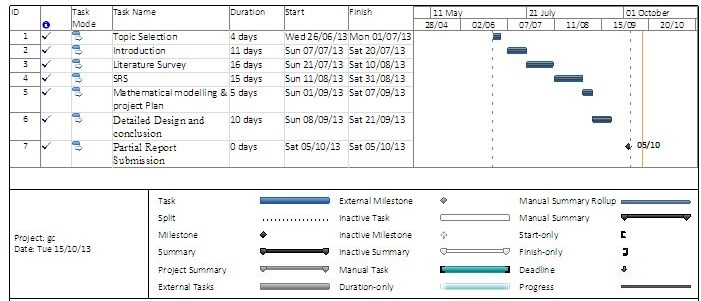
\includegraphics[width=17cm,height=13cm]{fig34.png}
  \caption{Gantt Chart of Scheduling of Sem I}\label{Gantt Chart of Scheduling Sem I}
\end{figure}

\newpage
$ \bullet $ Gantt Chart of Scheduling for Semester II is as follows : \\
\begin{figure}[h]
\centering
  % Requires \usepackage{graphicx}
  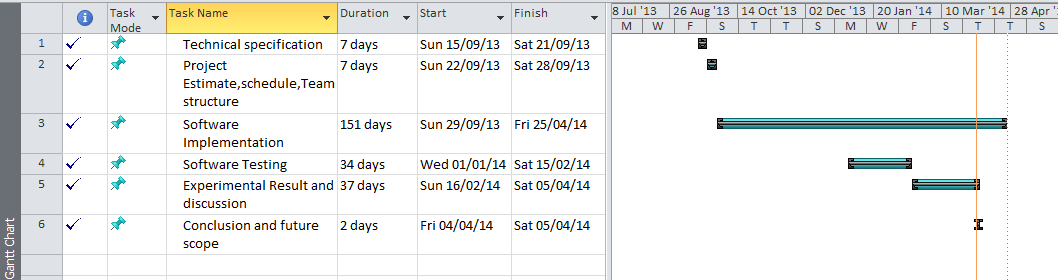
\includegraphics[width=14cm,height=7cm]{fig34-1.png}
  \caption{Gantt Chart of Scheduling Sem II}\label{Gantt Chart of Scheduling Sem II}
\end{figure}

\section{Feasibility Study}
\subsection{COCOMO Model}
Constructive cost model is one of the most widely used and discussed software cost estimation model. The Query by example based Video Retrieval System uses COCOMO MODEL. The basic COCOMO MODEL computes software development efforts and cost as a function of program size express in estimated line of code.

\begin{table}[h]
\begin{flushleft}
\centering
\caption{Analysis and Estimation Cocomo model} \label{Analysis and Estimation Cocomo model}
\begin{tabular}{|c|p{2cm}|p{2cm}|p{2cm}|p{2cm}|} \hline
Software Project & $a_{b}$ & $b_{b}$ & $c_{b}$ & $d_{b}$ \\ \hline
 \textbf{Organic} & 2.4 & 1.05 & 2.5 & 0.38 \\ \hline
 Semi Detached & 3.0 & 1.12 & 2.5 & 0.35 \\ \hline
 Embedded & 3.6 & 1.20 & 2.5 & 0.32 \\ \hline
 \end{tabular}
 \end{flushleft}
 \end{table}

\textbf{"A Tool for Managing Key Values pair on Oracle NoSQL Database"} is an \emph{Organic} project. \\

\hspace*{0.7in} $\maltese$  Effort = $a_{b}KLOC^{b_{b}} $ \\
\hspace*{0.7in} $\maltese$  Duration = $ c_{b}KLOC^{d_{b}} $ \\

\begin{table}[h]
\begin{flushleft}
\centering
\caption{Calculation} \label{Calculation}
\begin{tabular}{|c|c|} \hline
Functions (Modules) & Estimated LOC  \\ \hline
Module 1 (Connection) & 60 \\ \hline
Module 2 (Operation Selection) & 1000 \\ \hline
Module 3 (Result) & 700 \\ \hline
Total & 1760 \\ \hline
 \end{tabular}
 \end{flushleft}
 \end{table}

 \begin{itemize}
   \item $a_{b}=2.4$
   \item $b_{b}=1.05$
   \item $c_{b}=2.5$
   \item $d_{b}=0.38$
   \item KLOC=1.76
\end{itemize}

$\maltese$  Effort = $a_{b}KLOC^{b_{b}}$ \\
\hspace*{0.10in} = 2.4 * $(1.76^{1.05})$ \\
\hspace*{0.10in} = 4.345 persons/month. \\
\\
$\maltese$  Duration  = $c_{b}KLOC^{d_{b}} $ \\
\hspace*{0.10in} = 2.5 * $(1.76^{0.38})$ \\
\hspace*{0.10in} = 3.1 months \\
\\
$\maltese$  Number  of  people recommended  = $\frac{Efforts}{Duration}$ \\
\hspace*{0.10in} = $\frac{4.345}{3.1}$ \\
\hspace*{0.10in} = 1.5 persons \\
\hspace*{0.10in} = $\sim$ 2 person \\
\\
\textbf{LOC based Estimation:} \\
\hspace*{0.5in} $ \diamond $ The average productivity for our product is : 600 LOC/Month \\
\hspace*{0.5in} $ \diamond $ The labour rate estimated is : Rs. 1000/- per month \\
\hspace*{0.5in} $ \diamond $ The cost per line of code is : approximately Rs. 6 \\
\hspace*{0.5in} $ \diamond $ Base on LOC estimated and historical productivity data, \textbf{Total estimated project cost is : Rs. 22560/-}
\newpage
\section{Team Structure}
The team structure for this project is as follows :
\begin{figure}[h]
\centering
  % Requires \usepackage{graphicx}
  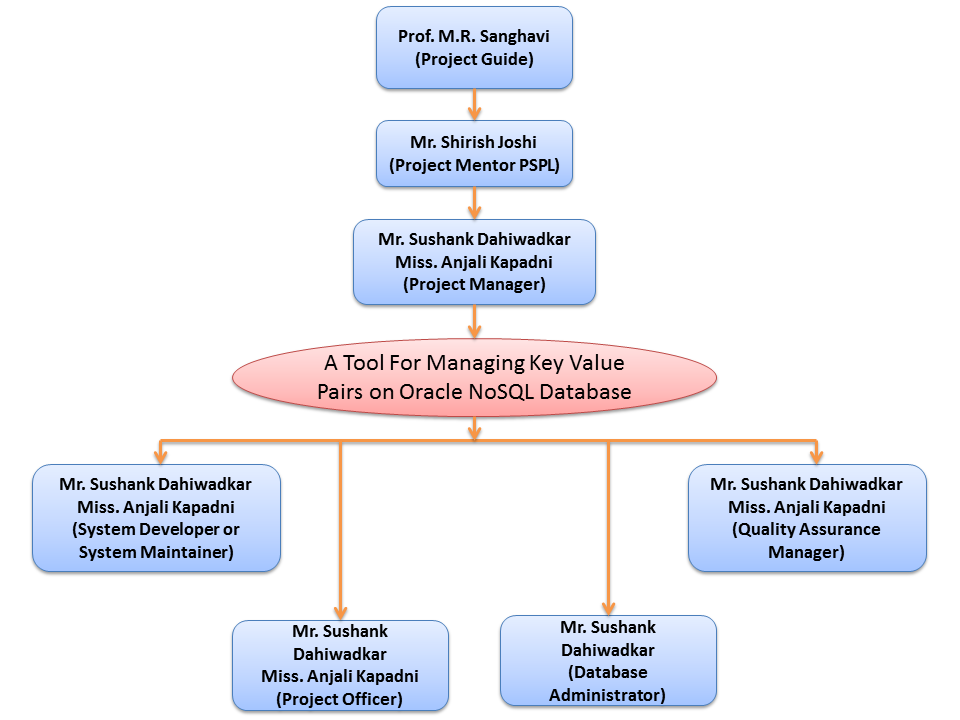
\includegraphics[width=15cm,height=15cm]{TS.png}\\
  \caption{Team Structure} \label{Team Structure}
\end{figure} 

\chapter{Software Implementation}
\section{System Implementation}
\begin{figure}[h]
\centering
  % Requires \usepackage{graphicx}
  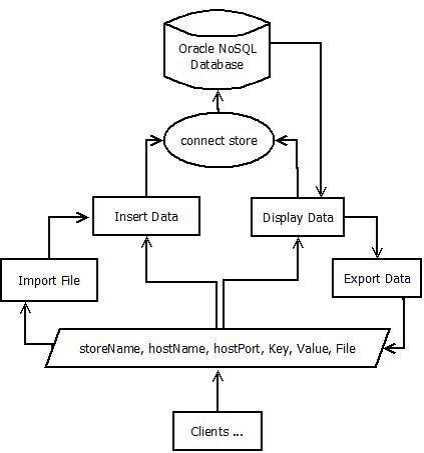
\includegraphics[width=12cm,height=10cm]{Fig21.jpg}\\
  \caption{System Architecture}
  \label{System Architecture}
\end{figure}
\begin{itemize}
  \item \textbf{Part1}
\end{itemize}
The system is a web application which fits into the application logic layer of three tier Architecture. System provides the ease to access key-value paired Oracle NoSQL database. System is a web interface through which the user can connect to the database and perform required operations. Position of the System in Three Tier Architecture is shown in figure
\\
\hspace*{0.7in} System's interface provides with various functionalities on database which includes CRUD operations and Import Export. The System follows disconnected architecture. in disconnected architecture the system is not synchronized with another system. System works in three stages i.e. connect to data store, perform operations and disconnect from data store. For performing every new operation the system needs to follow above three steps. System follows disconnected architecture then too system maintains session, in sessions Store Name, Host Name and Host Port are stored. Because foe every new operation user should not have to enter again those parameters.
\\
\hspace*{0.7in} The system interface is kept simple, so that any user having basic knowledge of key value based NoSQL database can use the system. The System is developed as a User Interface for Oracle NoSQL Database. System uses KVLITE which is a Single Node Data Store by Oracle NoSQL. The System uses kvclient.jar file which has all the necessary library files for using KVLITE or KVSTORE.
\\
Following operations can be performed using the Developed System:\\

\begin{enumerate}
  \item Connect to Store : \\
\hspace*{0.7in} This function connects the client to Data Store on Remote Server. this functions takes three parameters namely Store Name, Host Name i.e. host address on which the data store is installed and Host Port i.e. on which the Data Store's service is started. When the system connects to data store a new session is created and this session is maintained until the user completes specific operation or logs out from system.

  \item Insert Data : \\
\hspace*{0.7in} This function is used to insert Single or Multiple Key Value pairs in the Data Store. The function comes in two forms i.e. Single and Multiple Key Value Pair Insert. For Single Key Value Pair insert system requires three parameters, namely Major Key Component, Minor Key Component and Key Value. For Multi Key Value Pair Insertion the system first asks for Major Key Component and Minor Key Component Count, followed by that the user has to enter Minor Key Components and Key Values.

  \item Display Data : \\
\hspace*{0.7in} This function gets the data from the store and displays to user. Functions come in two forms i.e. Single and Multiple Key Value pair display. For Single Key Value display system takes Major Key and Minor Key Component and parameters. And for Multi Key Value pair display System takes only Major Key Value Component.

  \item Update Data : \\
\hspace*{0.7in} This function is used to update the existing Key Value pairs. This function also comes in two forms Single and Multiple Key Value Pairs Update. For Single Key Value Pairs update user has to enter Major Key Component, Minor Key Component and Key Value. And for Multi Key Value pair update user has to enter one Common Major Key Component and its Minor Key Components along with Key Values.

  \item Delete Data : \\
\hspace*{0.7in} Delete functions is used to delete existing Key value Pairs. The function has two forms. The first form is Single Key Value Pair delete where user has to enter Major and Minor Key Component. And for Multiple Key Value pair delete user has to enter only Major Key Component.

  \item Import Data : \\
\hspace*{0.7in} The function provides Import functionality. Here the data can be imported from a Comma Separated value file into the database. Here firstly user has to upload a file to server which is to be imported into the data store. After the file is been uploaded the system ask user to mention Major Key Component and Minor Key Component for that file along with the Minor Key Part. Here the Minor Key Component is a composite form of Minor Key Component specified by the user and a field from CSV file. These two parts makes a new Minor Key which is used to identify the Key Value Pair uniquely. This approach is used so that the Relational Database can be mapped with NoSQL Database.

  \item Export Data : \\
\hspace*{0.7in} Here the data from database is directly exported into the CSV (Comma Separated Value) file. The data which is to be exported is firstly fetched from database and if user wish to export that data into file then that data is exported into the CSV file. This function is only available for multiple Key Value pairs Export.
\end{enumerate}

\begin{itemize}
  \item \textbf{Part2}
\end{itemize}
\hspace*{0.7in} The Part 2 of project consists of Creating Web Services to access the NoSQL database. Web services are developed so that the any client independent of any platform can access the database. Here in our application RESTful webservices are developed. RESTful, because this are stateless and lightweight. This web services are meant to access from mobile devices. \\
\hspace*{0.7in}	In our case to demonstrate the use application of big data, Sensor generated data is stored and is access from the KVStore. This sensor data is gathered from the Bio Metrics Thumb machine use for daily attendance record. \\
\hspace*{0.7in}	Here two web services are created:
\begin{enumerate}
    \item To get the daily attendance of user : \\
\hspace*{0.7in} Here User gets the date wise attendance report. The user has to enter his/her user id In/Out log and Date and Log in or Log out Time is displayed to the user.

    \item To get the monthly attendance of the user : \\
\hspace*{0.7in} Here user gets the month wise attendance report. The user has to enter his/her user id and the respective month and year and the monthly attendance is displayed by calculating it from working days.
\end{enumerate}

\begin{itemize}
  \item \textbf{Part3}
\end{itemize}
\hspace*{0.7in} Android application is been developed through which the user gets his/her attendance report. The above explained web services are been consumed using this application.


\section{Mathematical Modeling and algorithm}
This mathematical model represents the proposed system described in the previous section.
$\bigodot S=\{\Sigma,q0,\delta,F,Q\} $ \\
Where \\
$\Sigma = \{ $ storeName, hostName, hostPort, majorKeyComponent, minorKeyComponent,  keyValue $\}$ \\
q0 = {Connect to Store} \\
$\delta$ = {f1 , f2 , f3 , f4 , f5 , f6 , f7} \\
f1= connectStore \\
f2 = insertSingleData \\
f3 = insertMultiData \\
f4 = displaySingleData \\
f5 = displayMultiData \\
f6= updateSingleRecord \\
f7= deleteSingleRecord \\
f8= deleteMultiRecord \\
f6 = importCSV \\
f7 = exportCSV \\
Q = {Connect to Store, Perform Operation, Disconnect from Store}
(All functions from f1 to f6 are already explained in previous section)


\subsection{Applications}
\begin{itemize}
  \item For managing key value paired oracle nosql database.
  \item For importing and exporting data from Oracle NoSQL Database.
  \item For attendance check to employees in organizations.
  \item The GUI based application can be used anywhere, where Oracle NoSQL databse comes into focus.
\end{itemize}

\subsection{Advantages and Disvantages}
\begin{itemize}
  \item Reduces efforts and time of user for managing Oracle NoSQL Database.
  \item Direct Import Export Functionality.
  \item REST Ful web services whose functionalities can be extended on any platform for any use.
\end{itemize}


\chapter{Software Testing}
\section{Introduction to Testing}
\hspace*{0.7in} The purpose of testing is to discover errors. Testing is the process of trying to discover every conceivable fault or weakness in a work product. It provides a way to check the functionality of components, sub-assemblies, assemblies and/or a finished product It is the process of exercising software with the intent of ensuring that the
Software system meets its requirements and user expectations and does not fail in an unacceptable manner. There are various types of test. Each test type addresses a specific testing requirement.
\subsection{Types of Tests}
\begin{itemize}
  \item \textbf{Level of Testing}
\end{itemize}
\begin{enumerate}
  \item Unit testing tests the minimal software component or modules. Each unit of the software is tested to verify that the details designed for unit has been correctly implemented.
  \item Integration testing exposes defects in the interface and interaction between integrated components. Progressively larger groups of tested software components corresponding to elements of architectural design are integrated and tested until the software works as whole.
  \item System testing tests an integrated system to verify that it meets its requirements.
  \item System integration testing verifies that system is integrated to any external or third party systems defined in the system requirements.
  \item Acceptance testing can be conducted by the end users customers of client to validate whether or not to accept the product. Acceptance testing may be performed after the testing and the before the implementation phase.
  \item Alpha testing is simulated or actual operational testing by potential users/customers or an independent test team at developers site. Alpha testing is often employed for off-the-shelf software as a form of internal acceptance testing, before the software goes to beta testing.
  \item Beta testing comes after alpha testing. Versions of the software, known as beta versions, are released to limited audience outside of the company. The software is released to the groups of people so that further testing can ensure the product has few faults and bugs. Sometimes, beta versions are made available to open public to increase the feedback field to maximal number of future users.
\end{enumerate}

\hspace*{0.7in} As a tester, it is always advisable to use manual white box testing and black box testing techniques on the test software. Manual testing helps discover and record any software bug or discrepancies related to the functionality of the product.
\\
\hspace*{0.7in} Manual testing can be replaced by test automation. It is possible to record and playback manual steps and write automated test script(s) using test automation tools. Although, Test automation tools will only help execute test scripts written primarily for executing a particular specification and functionality. Test automation tools lack the ability of decision-making and recording any unscripted discrepancies during program execution. It is recommended that one should perform manual testing of the entire product at least a couple of times before actually deciding to automate the more mundane activities of the product.
\\
\hspace*{0.7in} Manual testing helps discover defects related to the usability testing and GUI testing area. While performing manual tests the software application can be validated whether it meets the various standards defined for effective and effective usage and accessibility. For example, the standard location of the OK button on the screen is on the left and of CANCEL button on the right. During manual testing you might discover that on some screen, it is not. This is a new defect related to usability of screen.
\\
\hspace*{0.3in} A manual tester would typically perform the following steps for manual testing:
\begin{itemize}
  \item  Understand the functionality of program
  \item	 Prepare a test environment
  \item  Execute test case(s) manually
  \item  Verify the actual result
  \item  Record the result as PASS or FAIL
  \item  Make a summary report of the PASS and FAIL test cases
  \item  Publish the report
  \item  Record any new defects uncovered during the test case execution
\end{itemize}

\hspace*{0.7in}There is no complete substitute for manual testing. Manual testing is crucial for testing software application more thoroughly. Test automation has become a necessity mainly due to shorter deadline for performing test activities, such as regression testing, performance testing and load testing.

\section{Manual Test Cases}
\hspace*{0.7in}Following question answering provides an overview referred from the test plan built for the project being implemented:

\begin{table}[h]
\begin{flushleft}
\caption{test cases for connect to store}\label{test cases for connect to store}
\begin{tabular}{|p{1cm}|p{4cm}|p{4cm}|p{5cm}|} \hline
Sr.No. & Test Cases & Expected Results & Actual results \\ \hline
1 & Blank Store Name, Host Name and Host Port & Error Message: "Must Enter Store Name, Host Name and Host Port" & Error Message: "Must Enter Store Name, Host Name and Host Port" \\	 \hline
2 & Blank Store Name, Incorrect/Correct Host Name and Host Port  & Error Message: "Must Enter Store Name" & Error Message: "Must Enter Store Name, Host Name and Host Port" \\	 \hline
3 & Blank Host Name, Incorrect/Correct Store Name and Host Port & Error Message: "Must Enter Host Name" & Error Message: "Must Enter Store Name, Host Name and Host Port"\\	 \hline
4 & Blank Host Port, Incorrect/Correct Store Name and Host Name & Error Message: "Must Enter Host Name" & Error Message: "Must Enter Store Name, Host Name and Host Port"\\	 \hline
5 & Incorrect Store Name, Correct Host Name and Host Port & Error Message: "Enter Correct Store Name" & Error Message: "Cannot Connect to Store"\\	 \hline
6 & Incorrect Host Name, Correct Store Name and Host Port & Error Message: "Enter Correct Host Name" & Error Message: "Cannot Connect to Store"\\	 \hline
7 & Incorrect Host Port, Correct Store Name and Host Name & Error Message: "Enter Correct Host Port" &Error Message: "Cannot Connect to Store" \\	 \hline
8 & Incorrect Store Name, Host Name and Correct Host Port & Error Message: "Enter Correct Store Name and Host Name" & Error Message: "Cannot Connect to Store"\\	 \hline
9 & Incorrect Store Name, Host Port and Correct Host Name & Error Message: "Enter Correct Store Name and Host Port" & Error Message: "Cannot Connect to Store"\\	 \hline
10 & Incorrect Host Name, Host Port and Correct Store Name & Error Message: "Enter Correct Host Name and Host Port" &Error Message: "Cannot Connect to Store" \\	 \hline
11 & Incorrect Store Name, Host Name and Host Port & Error Message: "Enter Correct Store Name, Host Name and Host Port" & Error Message: "Cannot Connect to Store"\\	 \hline
12 & Correct Store Name, Host Name and Hot Port & Message: "Welcome to KVStore" & Message: "Welcome to KVStore"\\	 \hline
\end{tabular}
\end{flushleft}
\end{table}


\begin{table}[h]
\begin{flushleft}
\caption{test cases for Insert Data}\label{test cases for Insert Data}
\begin{tabular}{|p{1cm}|p{4cm}|p{4cm}|p{5cm}|} \hline
Sr.No. & Test Cases & Expected Results & Actual results \\ \hline
1 & Blank Major Key Component, Minor Key Component and Key Value & Error Message: "Please Enter all Parameters" & Error Message: "Data Insertion Failed"\\	 \hline
2 & Blank Major Key Component and Valid Minor Key Component and Key Value & Error Message: "Please Enter Major Key Component" & Error Message: "Please Enter all Parameters"\\	 \hline
3 & Blank Minor Key Component and Valid Major Key Component and Key Value & Error Message: "Please Enter Minor Key Component" & Error Message: "Please Enter all Parameters"\\	 \hline
4 & Blank Key Value and Valid Major Key Component and Minor Key Component & Error Message: "Please Enter Key Value" & Message: "Data Inserted Successfully"\\	 \hline
5 & Valid Major Key Component, Minor Key Component and Key Value & Message: " Data Inserted Successfully" & Message: "Data Inserted Successfully"\\	 \hline
 \end{tabular}
\end{flushleft}
\end{table}

\begin{table}[h]
\begin{flushleft}
\caption{test cases for Display Data}\label{test cases for Display Data}
\begin{tabular}{|p{1cm}|p{4cm}|p{4cm}|p{5cm}|} \hline
Sr.No. & Test Cases & Expected Results & Actual results \\ \hline
1 & Blank Major and Minor Key Component & Error Message: "Please Enter All Parameters" & Error Message: "Error"\\	 \hline
2 & Blank Major Key Component and Valid Minor Key Component & Error Message: "Please Enter All Parameters" & Error Message: "Please Enter All Parameters"\\	 \hline
3 & Blank Minor Key Component and Valid Major Key Component & Error Message: "Please Enter All Parameters" & Error Message: "Please Enter All Parameters" \\	 \hline
4 & Incorrect Major and Minor Key Component & Error Message: "Data not Available for given Parameters"  &Error Message: "Error" \\	 \hline
5 & Incorrect Major Key Component and Correct Minor Key Component & Error Message: "Data not Available for given Parameters"  & Error Message: "Error"\\	 \hline
6 & Incorrect Minor Key Component and Correct Major Key Component & Error Message: "Data not Available for given Parameters"  & Error Message: "Error"\\	 \hline
7 & Correct Major and Minor Key Component & Data Displayed & Data Displayed\\	 \hline
\end{tabular}
\end{flushleft}
\end{table}

\begin{table}[h]
\begin{flushleft}
\caption{test cases for Update Data}\label{test cases for Update Data}
\begin{tabular}{|p{1cm}|p{4cm}|p{4cm}|p{5cm}|} \hline
Sr.No. & Test Cases & Expected Results & Actual results \\ \hline
1 & Blank Major Key Component, Minor Key Component and Key Value & Error Message: "Please Enter all Parameters" & Error Message: "Data Insertion Failed"\\	 \hline
2 & Blank Major Key Component and Correct Minor Key Component and Key Value & Error Message: "Please Enter Major Key Component" & Error Message: "Please Enter all Parameters"\\	 \hline
3 & Blank Minor Key Component and Correct Major Key Component and Key Value & Error Message: "Please Enter Minor Key Component" & Error Message: "Please Enter all Parameters"\\	 \hline
4 & Blank Key Value and Correct Major Key Component and Minor Key Component & Error Message: "Please Enter Key Value" & Error Message: "Data Updation Failed"\\	 \hline
5 & Incorrect Major Key Component and Correct Minor key Component and Key Value & Error Message: "Please Enter Major Key Component" & Error Message: "Data Updation Failed"\\	 \hline
6 & Incorrect Minor Key Component and Correct Major key Component and Key value & Error Message: "Please Enter Minor Key Component" & Error Message: "Data Updation Failed"\\	 \hline
7 & Correct Major Key Component, Minor Key Component and Key Value & Message: " Data Updated Successfully" &Message: "Data Updated Successfully" \\	 \hline
\end{tabular}
\end{flushleft}
\end{table}

\begin{table}[h]
\begin{flushleft}
\caption{test cases for Delete Data}\label{test cases for Delete Data}
\begin{tabular}{|p{1cm}|p{4cm}|p{4cm}|p{5cm}|} \hline
Sr.No. & Test Cases & Expected Results & Actual results \\ \hline
1 & Blank Major Key and Minor Key Component & Error Message: "Please Enter all Parameters" & Error Message: "Error"\\	 \hline
2 & Blank Major Key Component and Valid Minor Key Component & Error Message: "Please Enter all Parameters" & Error Message: "Please Enter all Parameters"\\	 \hline
3 & Blank Minor Key Component and Valid Major Key Component & Error Message: "Please Enter all Parameters" & Error Message: "Please Enter all Parameters"\\	 \hline
4 & Incorrect Major Key Component and Correct Minor Key Component & Error Message: "Please Enter Correct Major Key Component" & Error Message: "Error"\\	 \hline
5 & Incorrect Minor Key Component and Correct Major Key Component & Error Message: "Please Enter Correct Minor Key Component" & Error Message: "Error"\\	 \hline
6 & Correct Major and Minor Key Component & Message: "Data Deleted Successfully" & Message: "Data Deleted Successfully"\\	 \hline
\end{tabular}
\end{flushleft}
\end{table}

\begin{table}[h]
\begin{flushleft}
\caption{test cases for Import Data}\label{test cases for Import Data}
\begin{tabular}{|p{1cm}|p{4cm}|p{4cm}|p{5cm}|} \hline
Sr.No. & Test Cases & Expected Results & Actual results \\ \hline
1 & Blank Select File Option & Error Message: "Please Select File" & Error Message: "Please Select Valid File"\\	 \hline
2 & Other than CSV file Selected & Error Message: "Please Select File" & Error Message: "Please Select Valid File"\\	 \hline
3 & Input CSV File & Message: "File Uploaded, Please Select Options for Import" & Message: "File Uploaded, Please Select Options for Import"\\	 \hline
4 & Blank Major, Minor Key Component and Minor Key Component Part Field & Error Message: "Please Enter all the Parameters" & Error Message: "Please Enter all the Parameters\\	 \hline
5 & Blank Major Key Component and Valid Minor Key Component and Minor Key Component Part Field & Error Message: "Please Enter all the Parameters" & Error Message: "Please Enter all the Parameters\\	 \hline
6 & Blank Minor Key Component and Valid Major Key Component and Minor Key Component Part Field & Error Message: "Please Enter all the Parameters" & Error Message: "Please Enter all the Parameters\\	 \hline
7 & Blank Minor Key Component Part Field and Valid Major Key Component and Minor Key Component & Error Message: "Please Enter all the Parameters & Error Message: "Please Enter all the Parameters\\	 \hline
8 & Valid Major, Minor Key Component and Minor Key Component Part Field & Message: "Data Imported Successfully" & Message: "Data Imported Successfully"\\	 \hline
\end{tabular}
\end{flushleft}
\end{table}

\begin{table}[t]
\begin{flushleft}
\caption{test cases for Export Data}\label{test cases for Export Data}
\begin{tabular}{|p{1cm}|p{4cm}|p{4cm}|p{5cm}|} \hline
Sr.No. & Test Cases & Expected Results & Actual results \\ \hline
1 & Blank Major Key Component & Error Message: "Please Enter Major Key Component" & Error Message: "Error"\\	 \hline
2 & Incorrect Major Key Component & Error Message: "Please Enter Major Key Component" & Error Message: "Error"\\	 \hline
3 & Correct Major Key Component & Data Displayed and File Download Option Appears & Data Displayed and File Download Option Appears\\	 \hline
\end{tabular}
\end{flushleft}
\end{table}


\chapter{Experimental Results And Discussion}
\hspace*{0.7in} Graphical user interface is designed and which is expressed through some screen shots using HTML and Java. The experiments carried out with the system are shown below with the help of graphical user interface of the system.
\begin{figure}[h]
\centering
  % Requires \usepackage{graphicx}
  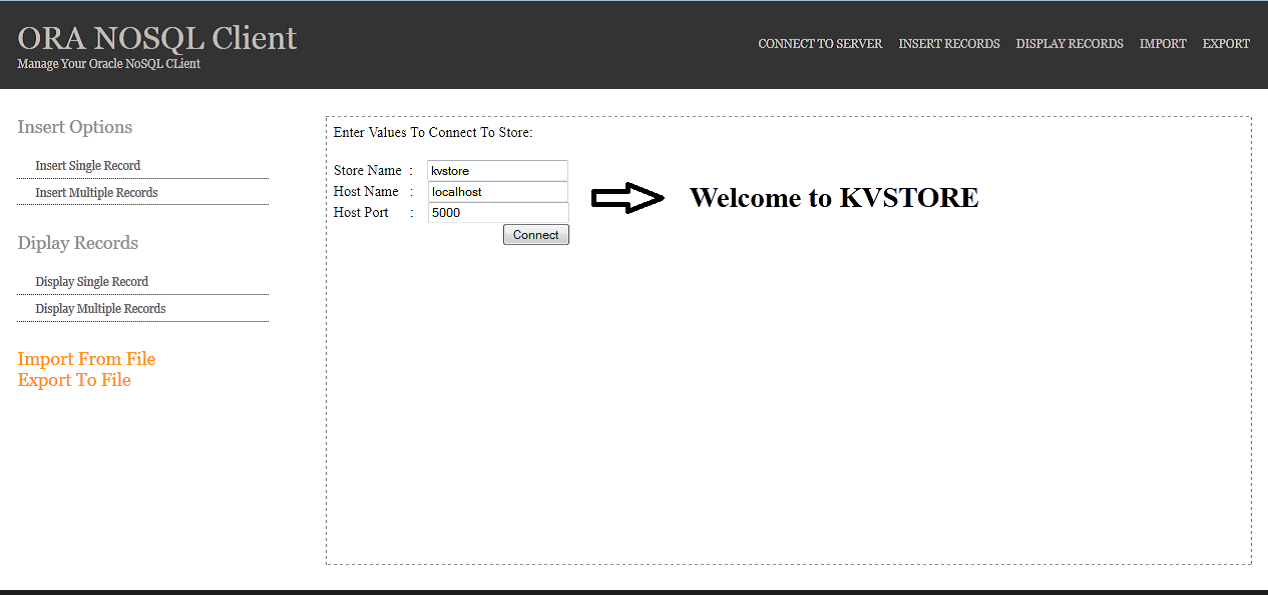
\includegraphics[width=13cm,height=7cm]{ERD1.png}
  \caption{Working Model of System.}\label{Working Model of System.}
\end{figure} \\
As the system was tested locally, it is capable of performing every operation listed above. The system is deployed on Glassfish Server and the results were good to compare with. Simultaneously various clients were connected and operations were performed and the System worked fine with that.\\

\newpage
\begin{figure}[h]
\centering
  % Requires \usepackage{graphicx}
  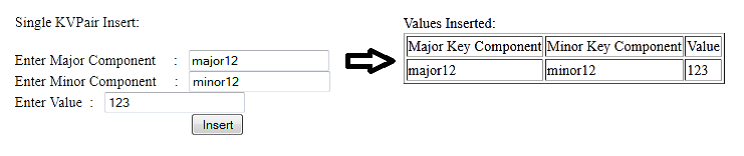
\includegraphics[width=13cm,height=3.5cm]{ERD2.png}
  \caption{Single KVPair Insert Operation}\label{Single KVPair Insert Operation}
\end{figure}
Above Figure shows Single KVPair insert and the same is applied for Multiple KVPair insert, but only first time the Major Key component and Number of Minor Key Components is asked and that number of fields is generated for user to insert value.

\begin{figure}[h]
\centering
  % Requires \usepackage{graphicx}
  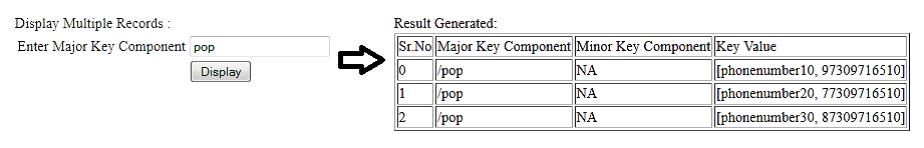
\includegraphics[width=13cm,height=3.5cm]{ERD3.png}
  \caption{Multiple KVPair Display Operation}\label{Multiple KVPair Display Operation.}
\end{figure}
Above Figure shows Multiple KVPair Display operation, same applies for Single KVPair display, but there user has to specify Major as well as Minor Key Component.

\begin{figure}[h]
\centering
  % Requires \usepackage{graphicx}
  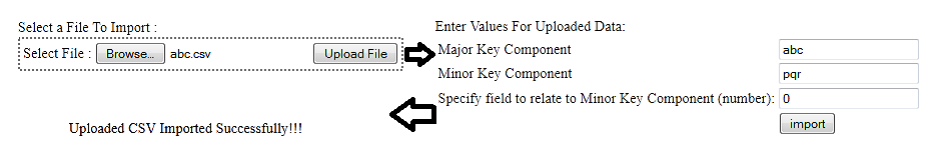
\includegraphics[width=13cm,height=3.5cm]{ERD4.png}
  \caption{Import CSV Operation.}\label{Import CSV Operation.}
\end{figure}
Above Figure shows Import Data from CSV operation, here the CSV file is uploaded to server and then user has to specify Major and Minor Key Component along with the index of field which is to be associated with Minor Key Component. \\
For Export Data to file, the user first has to perform Single or Multiple Display Operation and after that a link is provided, through which the user can download generated CSV file. \\ \\
Below are the Screen shots of Android Application, which is developed to consume the web services. This application is used for getting attendance report of the user.
\begin{figure}[h]
\centering
  % Requires \usepackage{graphicx}
  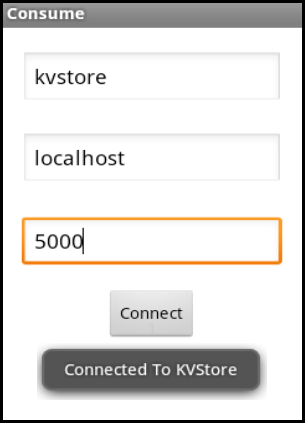
\includegraphics[width=6cm,height=7cm]{ERD5.png}
  \caption{Interface for connection to Store.}\label{Interface for connection to Store.}
\end{figure}
\\
\\
\\
\\
\begin{figure}[h]
\centering
  % Requires \usepackage{graphicx}
  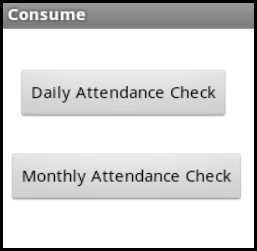
\includegraphics[width=6cm,height=7cm]{ERD6.png}
  \caption{Options for Attendance Check.}\label{Options for Attendance Check.}
\end{figure}

\newpage
\begin{figure}[h]
\centering
  % Requires \usepackage{graphicx}
  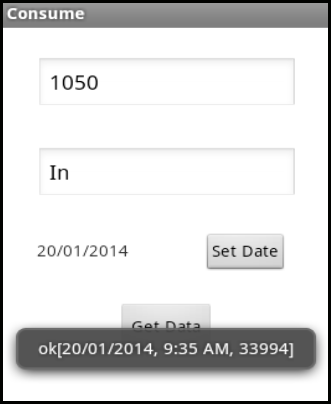
\includegraphics[width=6cm,height=7cm]{ERD7.png}
  \caption{Daily Attendance Check Interface.}\label{Daily Attendance Check Interface.}
\end{figure}

\begin{figure}[h]
\centering
  % Requires \usepackage{graphicx}
  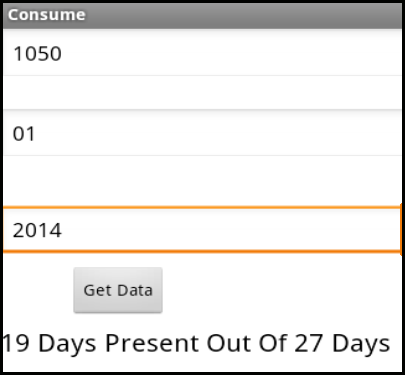
\includegraphics[width=6cm,height=7cm]{ERD8.png}
  \caption{Monthly Attendance Check Report.}\label{Monthly Attendance Check Report.}
\end{figure}
\hspace*{0.7in} In this way the experiments are carried out on every functions of the system and we have found various results as shown in above screenshots. The system works well. 



%\prefacesection{Conclusion And Future Scope}
\chapter{Conclusion And Future Scope}
\hspace*{0.7in}Understanding the need for managing BigData, a wide study is done of NoSQL Databases. Among which Oracle NoSQL Database was selected and it came into focus that, the Oracle NoSQL database is a fine tool to fulfill our needs, but Oracle NoSQL does not provide simplicity for na�ve users to utilize it. So this project is developed to manage the Oracle NoSQL Database by providing Graphical User Interface and Web Services to utilize the Oracle NoSQL facilities.
\\\hspace*{0.7in}The Project concentrates on Graphical User Interface to Manage the Key Value Pairs on Oracle NoSQL Database. The GUI developed in this project provides all the functions to manage the Oracle NoSQL Database. The System provides all CRUD operations and Import CSV and Export Data Facility. The System uses Disconnected Architecture.
\\\hspace*{0.7in}Further, RESTFul Web Services are developed which can be accessed from any platform. An Attendance Check application is developed for Android Platform, which demonstrates the use of Oracle NoSQL for managing Big Data. Here the BigData is taken as Sensor Data generated from Bio Metrics Thumb machine.
\\\hspace*{0.7in}The Future Scope includes developing a complete package of Web Services to use Oracle NoSQL Database.
\\\hspace*{0.7in}So, "A Tool for Managing Key Value Pairs on Oracle NoSQL Database" will definitely help all the users of Oracle NoSQL Database to utilize its all functionalities. And will encourage scholars to further study and develop the application.


\nocite{*}
\bibliographystyle{IEEEtran}
\bibliography{ref1}

\prefacesection{Appendix}
\begin{itemize}
  \item \textbf{Abbreviations:}
\end{itemize}

CRUD: Create, Read, Update, Delete.\\
CSV: Comma Separated Value.\\
GUI: Graphical User Interface.\\
HTTP: Hypertext Transfer Protocol.\\
IDE: Integrated Development Environment.\\
JSON: Java script Object Notation.\\
RDBMS: Relational Database Management System.\\
REST: Representational State Transfer.\\
SAN: Storage Area Network.\\
SQL: Structured Query Language.\\
UML: Unified Modeling Language.\\
XML: Extensible Markup Language.\\

\newpage
\begin{itemize}
  \item \textbf{Project Code:}
\end{itemize}

\prefacesection{Authors Profile}
\begin{figure}[h]
\centering
  % Requires \usepackage{graphicx}
  \includegraphics[width=17cm,height=16cm]{AP.png}
  \caption{Authors Profile}\label{Authors Profile}
\end{figure}



%Use following command at the command prompt to display the Index
% makeindex thesis
%%%%%\newpage
%%%%%\addcontentsline{toc}{chapter}{Index}
%%%%%\printindex

\end{document}

